\documentclass[hidelinks,11pt]{article}
\usepackage{fullpage}
\usepackage{amsfonts}
\usepackage{amssymb}
\usepackage{amsmath}
\usepackage{hyperref}
\usepackage{titling}
\usepackage{color}
\usepackage{graphicx}
\usepackage{fancyhdr}   
\usepackage{float}
\usepackage[top=1.0in, bottom=1.0in, left=1.0in, right=1.0in]{geometry}
\usepackage[font=small,justification=justified, format=hang]{caption}
\usepackage[utf8]{inputenc}
\usepackage[english]{babel}
\usepackage{xspace}
\usepackage{wrapfig}
\usepackage{hyperref}
\usepackage{authblk}
\setlength\parindent{0pt}
%\usepackage{lineno}
%\linenumbers

\numberwithin{figure}{section}
\numberwithin{table}{section}

\newcommand{\degree}{\mbox{$^\circ$}\xspace}

%new commands
%\newcommand{\eta}{\mbox{$\eta}\xspace}
%\newcommand{\phi}{\mbox{$\phi}\xspace}


\begin{document}

\title{T1044-2017 and 2018 sPHENIX Test Beam EMCal Position Scan Analysis}
\author[1]{Zhaozhong Shi}
\author[2]{Jin Huang}
\affil[1]{MIT}
\affil[2]{Brookhaven National Laboratory}

\date{\today}

% sPH-CALO-2018-XXX

% \begin{center}
% 	{\LARGE T1044-2018 sPHENIX Test Beam EMCal Analysis}\\
%     \vspace{1cm}
%     {\large Joe Osborn$^1$ and Jin Huang$^2$\\}
%     \vspace{0.5cm}
%     {\large $^1$ University of Michigan \\
%     $^2$Brookhaven National Laboratory\\}
%     \vspace{0.5cm}
%     {\large November 7, 2017}
    
% \end{center}
\maketitle


\begin{abstract}
sPHENIX Collaboration conducted test beam experiment at Fermilab Test Beam Facilities in 2017 and 2018 to study the performance of the sPHENIX calorimeter systems. The sPHENIX calorimeter systems consist of electromagnetic calorimeter (EMCal) and inner and outer hadronic calorimeter (HCAL). We have conducted energy and position scan to study the uniformity, energy linearity, and energy resolution of the calorimeter systems. In this paper, we will present our detailed analysis on the 2017 and 2018 EMCal position scans to study its uniformity and discuss the possible methods to improve the EMCal uniformity.
\end{abstract}


\tableofcontents

\clearpage
\listoffigures
\clearpage
%\listoftables
%\clearpage


\setlength{\parskip}{1em}




\section{Introduction}

\subsection{Motivation}

The sPHENIX EMCal plays an important role on the sPHENIX physics analyses. It is crucial for the following physics analyses \cite{sPHENIXPaper}: 

1. Identifying electron from decay of Upsilon states, which serve as a thermometer for QGP

2. Detecting photon in photon-jet pair productions, which tag the initial kinematics of the partons that initiate the jets

Therefore, in the test beam experiments, we conduct position scans of the EMCal towers to understand the uniformity and find possible solutions to improve its uniformity from our studies. 

\subsection{2017 Test Beam Run}

The 2017 T-1044 test beam run is designed to be the first test of the high rapidity $\eta\sim$1 sPHENIX calorimetry. In particular, the EMCal tested was the first with 2D projective tungsten scintillating fiber towers produced, and thus the test beam was a first step in understanding the 2D projective towers. It is also the first sPHENIX test beam with blocks containing the 2 $\times$ 2 tower configuration that sPHENIX intends to build. Nearly all of the test beam details are documented in the wikipedia page:

\url{https://wiki.bnl.gov/sPHENIX/index.php/2017\_calorimeter\_beam\_test}

\noindent Since this was the first high rapidity EMCal, there was emphasis in the data collection to study and understand the effects of the block boundaries. The effect of the block boundaries was quantified by performing energy scans covering either one single tower and several towers to include the effects of the block boundaries. To quantify these effects, position dependent energy responses were made for these runs. These responses could then be used as recalibration to the overall energy response, depending on where the electron showered. %This procedure will be documented here, in addition to the various analysis cuts and methods used to construct final results. 




\subsection{2018 Test Beam Run}

The 2018 T-1044 test beam run is designed to test more realistic positioning at high rapidity ($\eta \sim 1$) of the sPHENIX detector with the improvement of our studies from the 2017 test beam run. We study the EMCal at three different orientations: dual channeling ($0 \degree$ tilted in the horizontal and vertical directions), sPHENIX rotation ($5 \degree$ tilted in the horizontal and vertical directions), and sPHENIX+5 rotation ($10 \degree$ tilted in the horizontal and vertical directions). We will also compare our results with the 2017 results in this document. The detailed of the 2018 test beam run can be found on the wikipedia page: 

\url{https://wiki.bnl.gov/sPHENIX/index.php/T-1044-2018}



The photos of the 2017 and 2018 test beam setup are shown on Figure~\ref{fig:TestBeam} below

\begin{figure}[hbtp]
\begin{center}
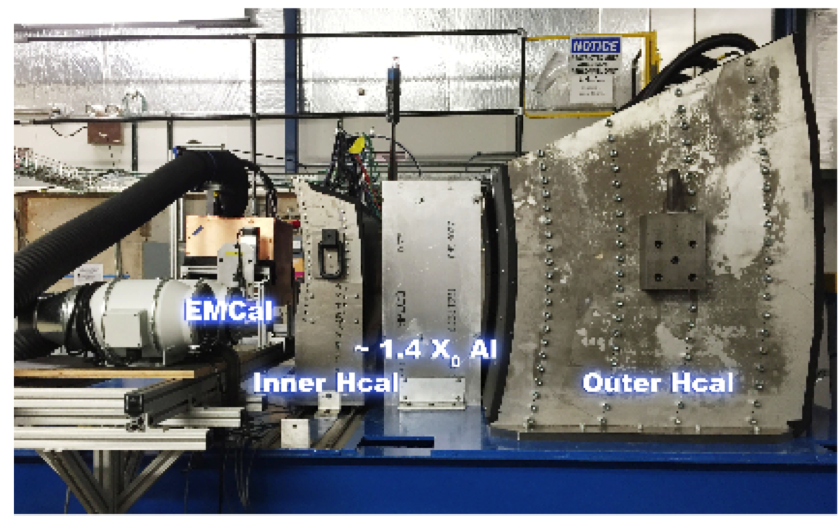
\includegraphics[width=0.30\textwidth]{Plots/TestBeamPhotos/2017TestBeamSetup.png}
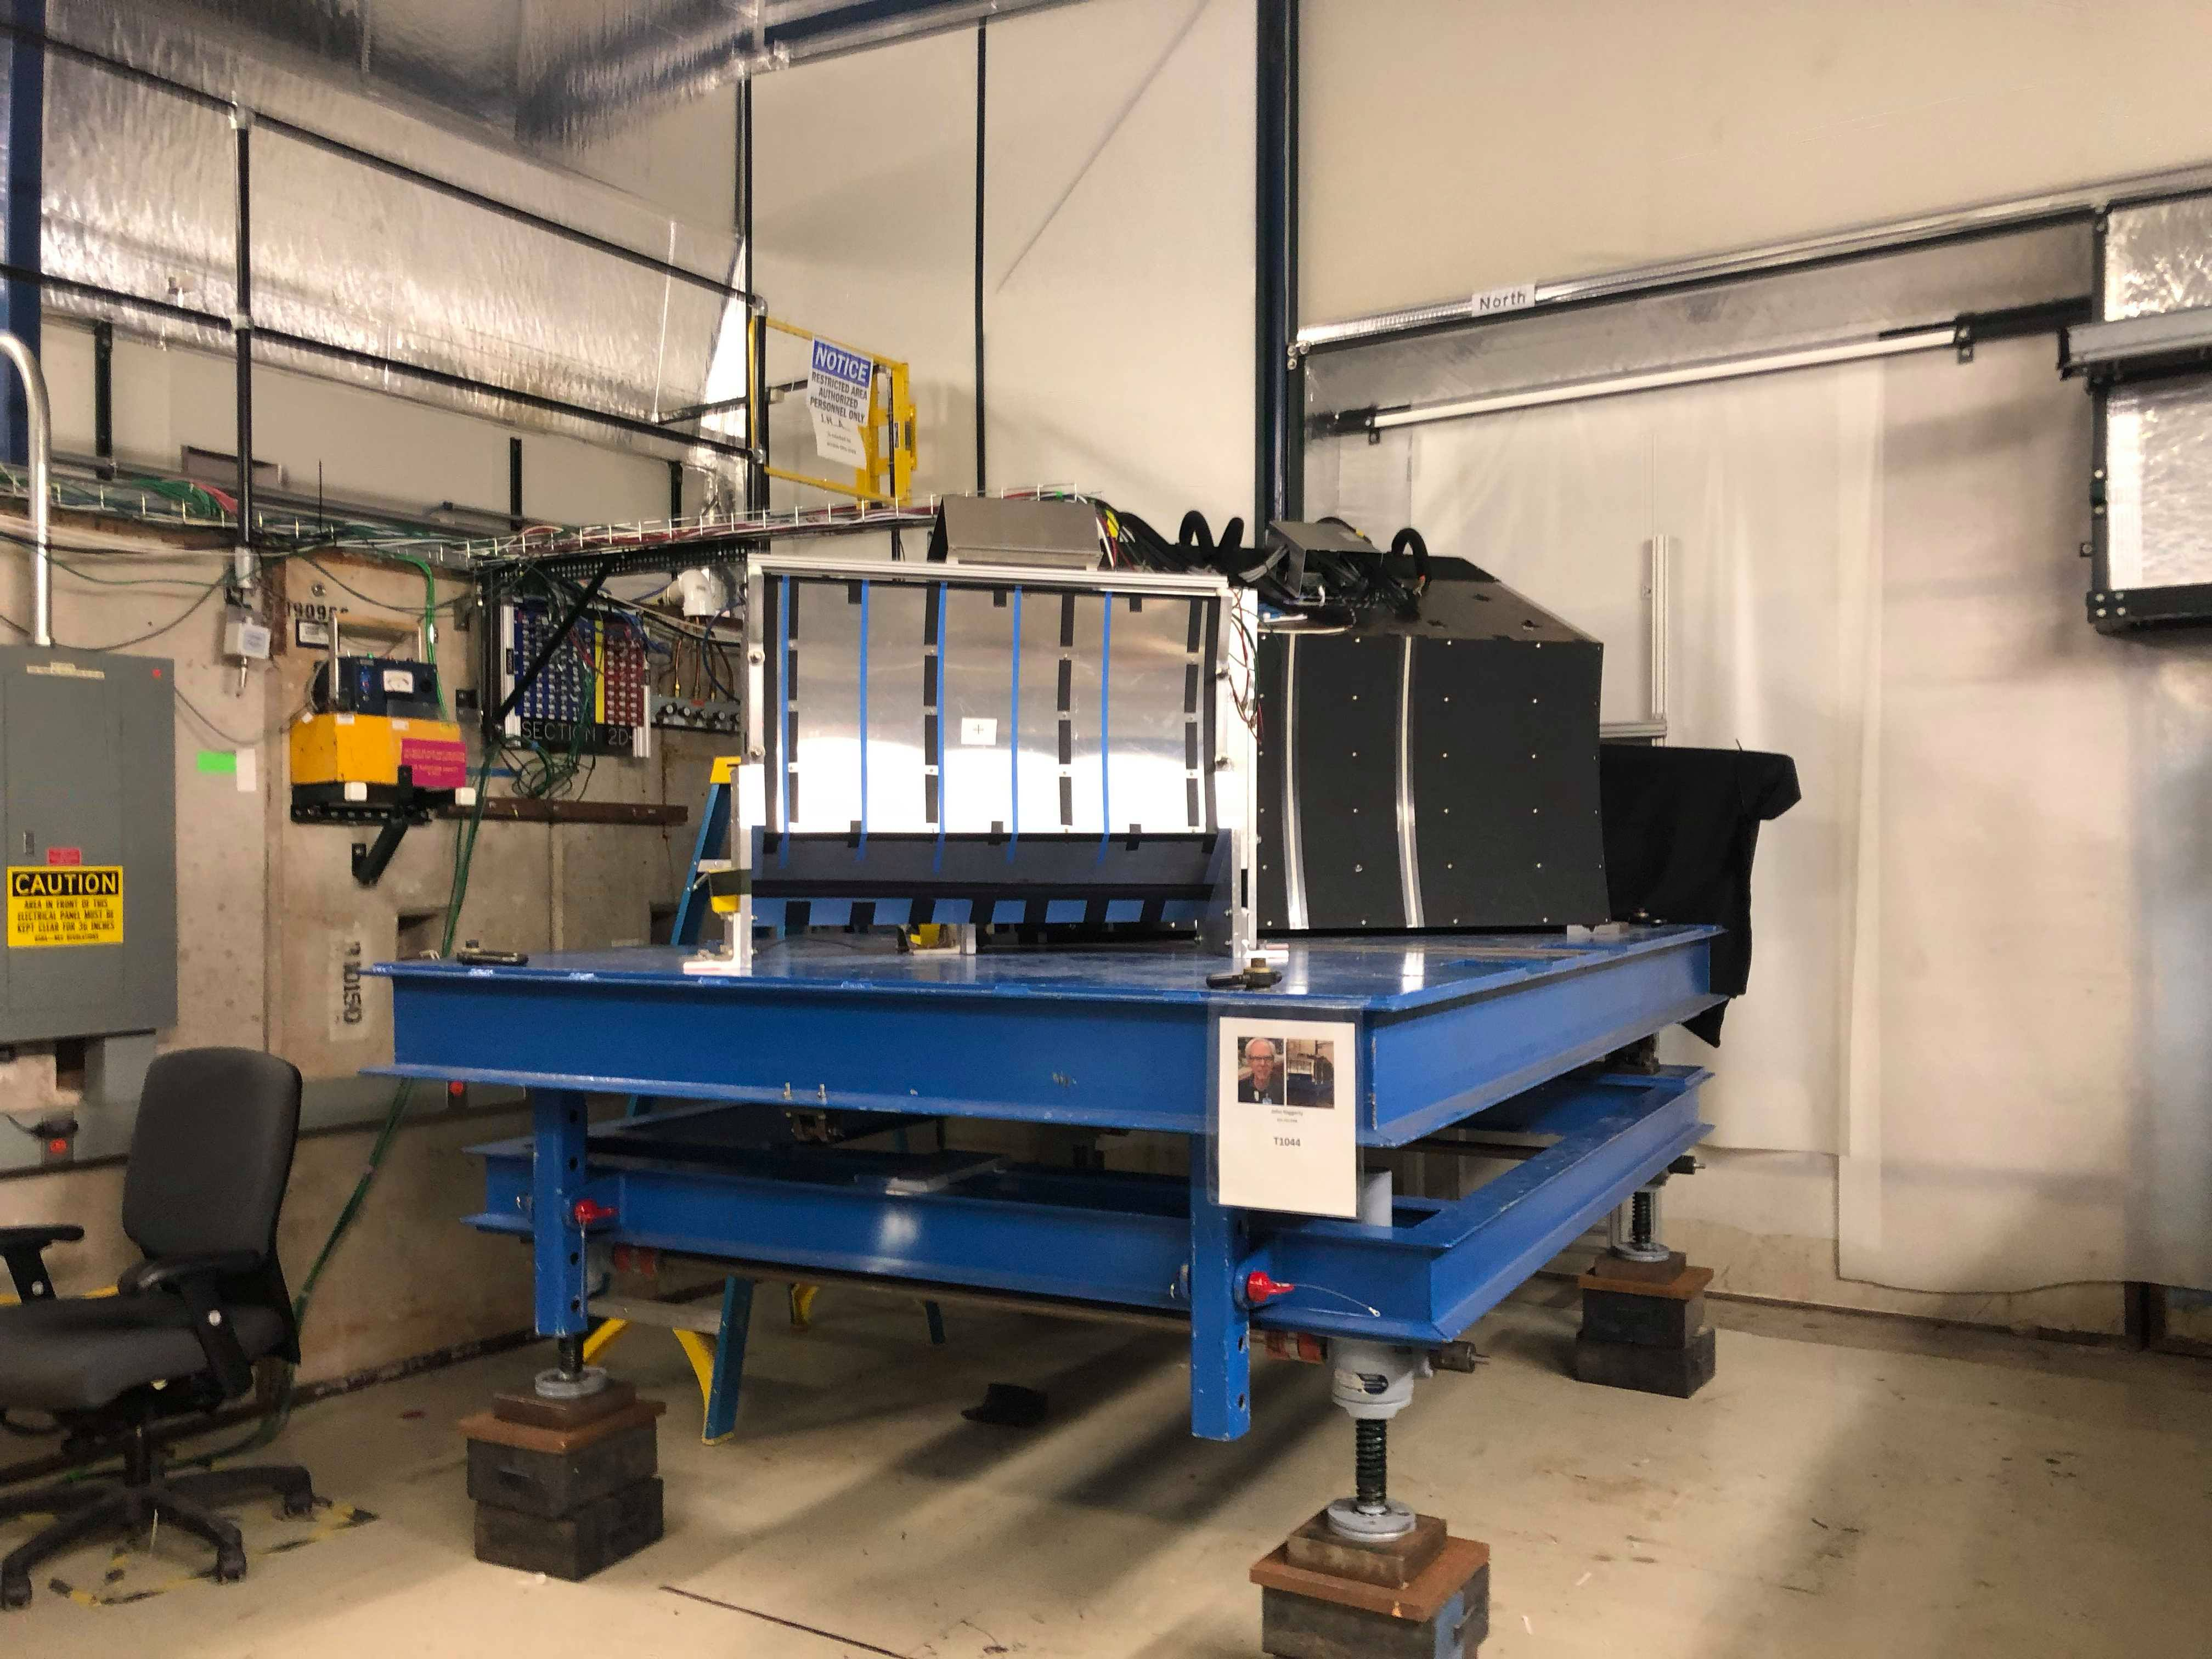
\includegraphics[width=0.25\textwidth]{Plots/TestBeamPhotos/2018TestBeamSetup.png}
\caption{Figure~\ref{fig:TestBeam} shows the 2017 (January to February 2017, left) and first 2018 test beam run (February to March 2018, right) respectfully for the sPHENIX calorimeters, both positioned at $\eta \sim$ 1, at Fermilab Test Beam Facilities.}
\label{fig:TestBeam}
\end{center}
\end{figure} 


We should note that we have three separate test beam runs in the 2018 test beam due to the schedule. In addition, our studies from the test beam on the EMCAL will be very helpful for us to develop calorimeter systems for experiments at the future Electro-Ion Collider. 


\section{Software Documentation}

Wikipedia pages documenting test beam information and analysis can be found at Refs.~\cite{beamtestwiki}. A wikipedia page documenting various EMCal meeting presentations and other information regarding the 2017 EMCal analysis can be found at Ref.~\cite{EMCALMeetings}. The code used for this analysis is located in the sPHENIX github repository. General codes for sPHENIX test beam data analysis can be found in Ref.~\cite{sPHENIXgithub} and the EMCAL position scan analysi can be found  Ref.~\cite{MyCodesgithub}. Code and macros used for analyzing the data and constructing the position dependent corrections can be found in the subsequent directories within github in ShowerCalib/ and ShowerCalib\_PositionDependent/. 

\noindent It should also be noted that the position dependent energy correction is the same as what was implemented in the full sPHENIX barrel simulations. This acts on the clusters after the initial clustering calibration, and can be found in the sPHENIX github repository~\cite{sPHENIXgithub}. 

\section{Data Acquisition, Production, and Calibration}

\subsection{Position Scan Data Acquisition}

The table of the EMCal at the test beam center moves much faster horizontally than vertically. Therefore, we make snake-like scan path for each tower horizontally and go vertically up when each horizontal. We create a lists of position for each run and make the script to move table according to our list. The scanning path for 2017 and 2018 test beam are shown as follows in Figure~\ref{fig:scanpath}.

\begin{figure}[hbtp]
\begin{center}
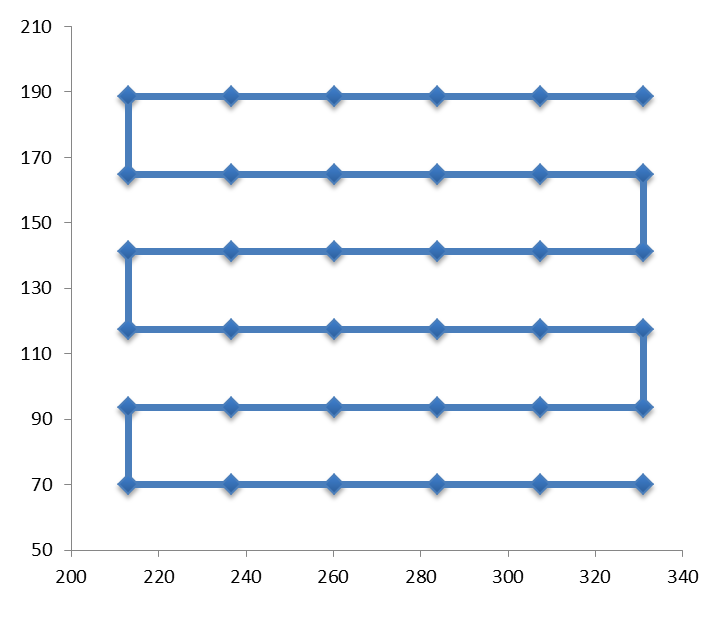
\includegraphics[width=0.30\textwidth]{Plots/2017ScanPath.png}
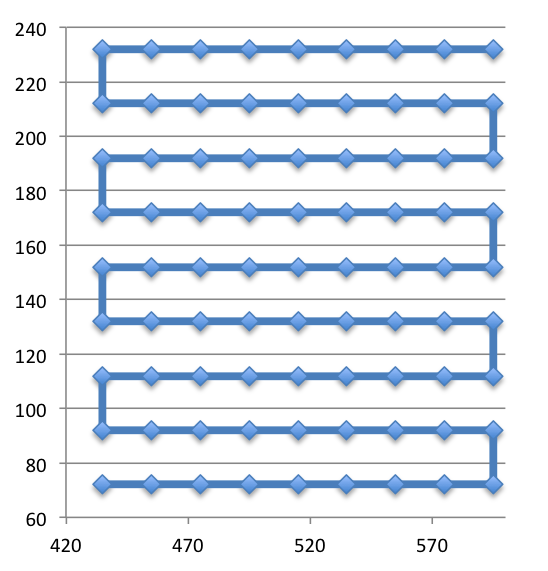
\includegraphics[width=0.25\textwidth]{Plots/2018ScanPath.png}
\caption{The position scan path plots for 2017 (left) and 2018 (right) test beam runs are shown above.}
\label{fig:scanpath}
\end{center}
\end{figure} 

The data are acquired in the format of prdf and are then converted into root files (RCDAQ developed by Martin Purschke \cite{RCDAQ}). Zhaozhong Shi, Murad Sarsour, Sean Stoll participate in position scan data taking in 2017 test beam. Zhaozhong Shi, Xu Sun, Sean Stoll and Murad Sarsour participate in 2018 test beam run. 

\subsection{2017 Test Beam Data}

In our 2017 test beam run, we have conducted three position scans at $\eta \sim 1$. In the first and second position scans, the EMCal is tilted at $10 \degree$ in the horizontal and vertical positions. In the third position scan, the EMCal is tilted at $0 \degree$. Cherenkov counter is used in the second and third position scans but not used in the first position scan. We measure the energy deposition of 8 GeV electron beams on the different positions of 6 $\times$ 6 EMCal towers for one tower per run (total 36 runs) and extract the mean energy from energy spectra. We also test the performance of 1-inch and 2-inch light guides in the position scan. Each run has a about 50000 events. The detail of the 2017 test beam run on EMCal position scan can be found on: 

\url{https://wiki.bnl.gov/sPHENIX/index.php/2017_calorimeter_beam_test/EMCal_runs_and_analysis}


\subsection{2018 Test Beam Data}

In our 2018 test beam run, we have conducted seven position scans at $\eta \sim 1$ from February to June. In the first test beam run, the beam is 4 GeV electron beam. In the first position scan, the EMCal is tilted at $5 \degree$ for both horizontal and vertical directions (sPHENIX rotation). We have total $8 \times 8 = 64$ and 50000 events for each run. In the second position scan, the EMCal is tilted at $0 \degree$ (dual channeling). We have total $8 \times 8 = 64$ and 25000 events for each run. Due to the dissatisfaction of our results on the position scan data, we then rerun a third preview run of sPHENIX rotation orientation. We have total $4 \times 4 = 16$ and 25000 events for each run. After that, we rerun the fourth sPHENIX rotation and fifth dual channeling, which have $9 \times 9 = 81$ runs with 2 cm increment horizontal/vertically between two consecutive runs. We study the rerun data and find that there is no significant improvement on the sPHENIX rotation compared to the $10 \degree$ tilted studies in the 2017 test beam run. Hence, subsequently, we conduct addition fifth, sixth, and seventh position scans in April, all of which have 81 runs. The beam for the second run is 8 GeV electron beam.  The fifth position scan is on dual channeling and has about 40000 events per run. The sixth position scan is on sPHENIX rotation + 5, which is about $10 \degree$ tilted for the EMCal just like the 2017 configuration. It has about 35000 events per run. The seventh position scan is on sPHENIX rotation and has about 27000 events per run. The detail of the 2018 test beam run on EMCal position scan can be found on:

\url{https://wiki.bnl.gov/sPHENIX/index.php/2018_calorimeter_beam_test/EMCal_runs_and_analysis}

\subsection{Dataset Used}

In this analysis notes, the second and third position scans in 2017 test beam and the third to seventh position scans in 2018 test beam taken at Fermilab Test Beam Facilities are used because of the high quality and statistics of the datasets. In the 2017 test beam run, we use ``clus$\_$5x5$\_$recalib", which stands for shower recalibration for the energy.  In the 2017 test beam run, we use ``clus$\_$5x5$\_$prod", which standard for shower production for the energy. The detail for the shower production and recalibration can be found at Jin Huang's slides \cite{Calib}.

\subsection{Dataset Production}

We run the codes located at \url{https://github.com/sPHENIX-Collaboration/analysis/tree/master/Prototype4/EMCal} to convert ``.prdf" format to ``.DSTReader.root" and then to ``.EMCalCalib.root" format with the options of either prod or recalib standing for standard shower calibration and recalibration respectfully. The detail instruction for compilation and run are documented on the sPHENIX webpage \url{https://wiki.bnl.gov/sPHENIX/index.php/2018_calorimeter_beam_test/Tutorial#Level_2:_formal_analysis_via_analysis_module}. The dataset we use in our analysis are the final readable root file format ``.EMCalCalib.root".


\subsection{Analysis Cuts }

To make sure that we have good quality of data, we apply ``good electrons" (good\_e) selections on the energy spectrum. This required that there be a valid hodoscope hit in both the vertical and horizontal fingers, or that in each direction the energy measured in the hodoscope was greater than a threshold ADC of 30. The ``good\_e" cut also required that the Cherenkov energy sum was greater than an energy threshold of 100 as a function of the truth electron beam energy. These cuts were utilized in order to suppress both background from MIPs as well as hadron contamination in the beam. After these cuts were implemented, a simple clustering algorithm was performed to determine the energy response as well as cluster $\phi,\eta$ position.


\noindent Clustering was performed with a simple algorithm. Both 3 $\times$ 3 and 5 $\times$ 5 clusters were constructed, where the 3 $\times$ 3 and 5 $\times$ 5 simply refer to the number of towers included in the clustering algorithm. The tower with the maximum energy was determined for a particular event. From that tower, the energy response was determined to be the total calibrated energy sum in a 3 $\times$ 3 or 5 $\times$ 5 tower square around the maximum energy tower. The cluster $\phi$ and $\eta$ position were determined with an energy weighted average in that 3 $\times$ 3 or 5 $\times$ 5 tower square. Calibrated tower energies were determined offline via MIP calibrations as was done in the previous 2016 test beam~\cite{OsbornNotes}. Recalibrated energies using the hodoscope or position dependence of the cluster are described in Jin Huang's slides \cite{Calib}. 

% Analysis cuts can be found in the code package /ShowerCalib/ as discussed above. The cuts are elaborated on here.

% Only runs that passed electron cuts were analyzed. The only cut which was required was that there be a ``good\_e'' cut, i.e. good electron. This required that there be a valid hodoscope hit in both the vertical and horizontal fingers, or that in each direction the energy measured in the hodoscope was greater than a threshold ADC of 30. The ``good\_e" cut also required that the Cherenkov energy sum was greater than an energy threshold of 100 as a function of the truth electron beam energy. These cuts were utilized in order to suppress both background from MIPs as well as hadron contamination in the beam. After these cuts were implemented, a simple clustering algorithm was performed to determine the energy response as well as cluster $\phi,\eta$ position.


% Clustering was performed with a simple algorithm. Both 3x3 and 5x5 clusters were constructed, where the 3x3 and 5x5 simply refer to the number of towers included in the clustering algorithm. The tower with the maximum energy was determined for a particular event. From that tower, the energy response was determined to be the total calibrated energy sum in a 3x3 or 5x5 tower square around the maximum energy tower. The cluster $\phi$ and $\eta$ position were determined with an energy weighted average in that 3x3 or 5x5 tower square. Calibrated tower energies were determined offline via MIP calibrations as was done in the previous 2016 test beam~\cite{Aidala:2017rvg}. Recalibrated energies using the hodoscope or position dependence of the cluster are described in further detail below.




%The hodoscope position dependent correction was first used in Ref.~\cite{Aidala:2017rvg}. 

%\begin{figure}[H]
%	\centering
%	\includegraphics[width=0.6\textwidth]{}
%	\caption{}
%	\label{}
%\end{figure}



%\section{Simulations}

%Simulations were performed with the default Prototype3 testbeam macro, located in \\/macros/macros/prototype3/. Small modifications to this macro will be discussed in the appropriate subsection. Single electron events were simulated using all Proto3 detectors. The beam characteristics were taken straight out of the {GitHub} macro. The beam included a 1 millirad angular divergence in both $\eta$ and $\phi$ space as well as a 2\% momentum smearing which are the same as the actual test beam. Gaussian vertex distributions were used as was in the git macro. A snippet of the code with the beam conditions can be found in the July 18 2017 EMCal presentation, for which links exist at the wiki pages from Section 2. One change that was made offline was to tilt the beam by 10 degrees for the first joint energy scan; this was to match the beam direction as it was in data. In the third joint energy scan, the beam direction was 0 degrees, i.e. square to the face of the calorimeter, so no modification was necessary. The tilt of the beam has important effects on both the positional energy response as well as the overall energy response of the detector, since the 10 degree beam tilt has more radiation lengths to traverse in the EMCal.


%\subsection{Simulation Results}


\section{Data Analysis}

\subsection{Hodoscope-Motion Table Calibration}

The hodoscope provides us precise measurement of the positions of the towers in the EMCal. We correct the horizontal and vertical position of beam on the EMCal with the $5 \times 5$ hodoscope fingers with $1 mm \times 1 mm$ position resolution. However, we do not know the sign of the hodoscope correction on the horizontal and vertical position. To figure out the sign for hodoscope correction, we plot all possible signs ($2 \times 2$) correction to the mean energy vs horizontal/vertical axis and look for a step-like pattern because of the EMCal block has a Cartesian structure. We find that the except the seventh position scan in 2018, the hodoscope sign are  ``-" for horizontal and ``+" for vertical positions. For the seventh position scan, the hodoscope sign are ``+" for horizontal and ``+" for vertical positions. Figure~\ref{fig:hodoCorr} show the hodoscope corrections plots for all 2017 and 2018 position scans:

\begin{figure}[hbtp]
\begin{center}
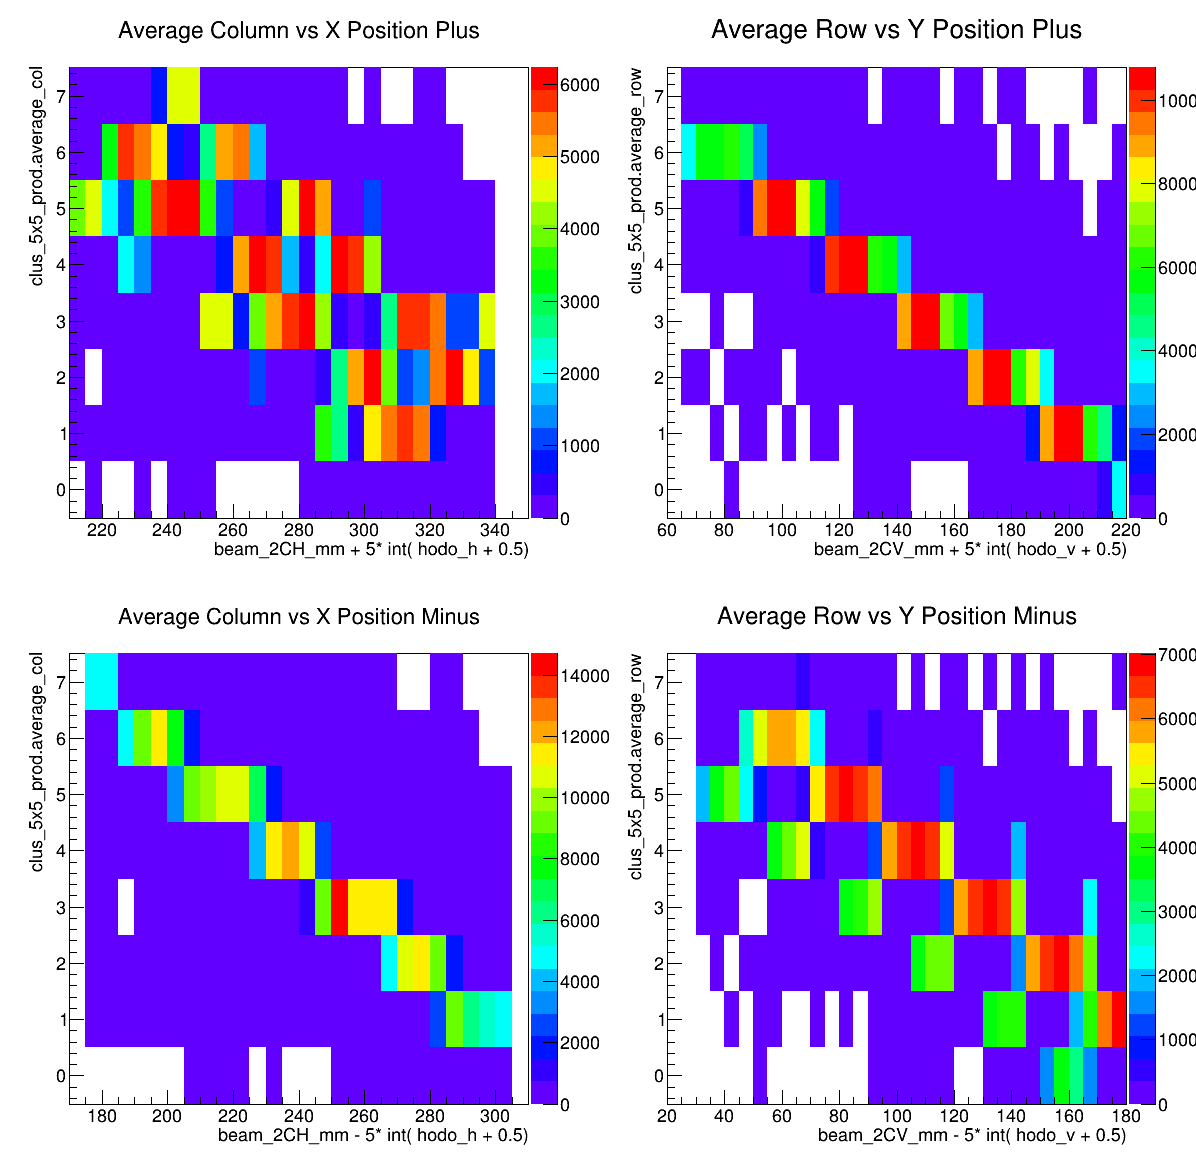
\includegraphics[width=0.38\textwidth]{Plots/Hodo/Hodoscope20172nd.png}
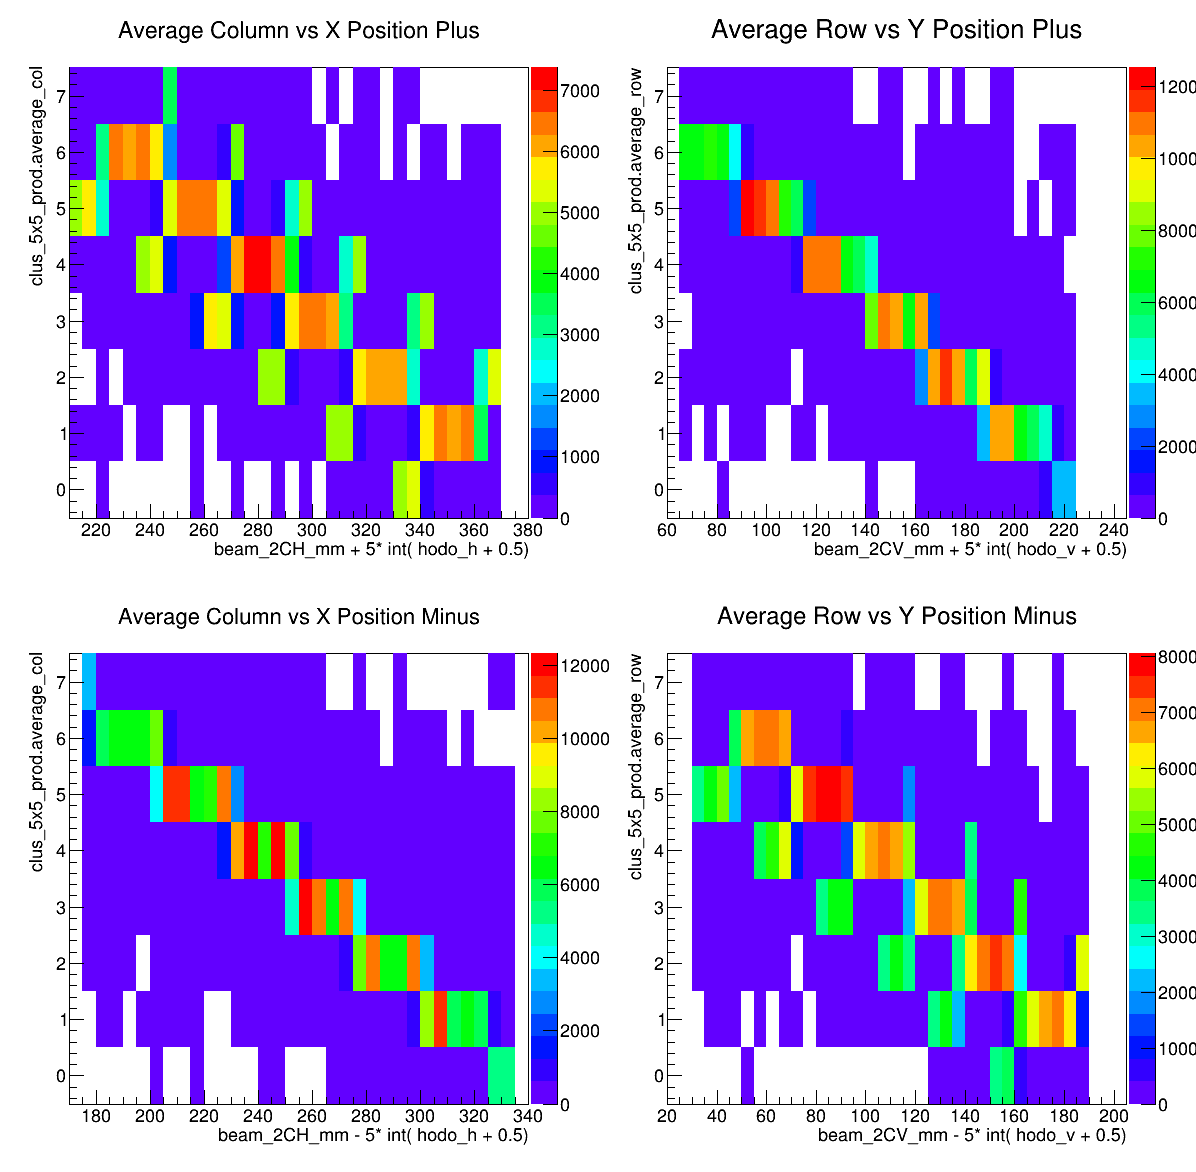
\includegraphics[width=0.38\textwidth]{Plots/Hodo/Hodoscope20173rd.png}
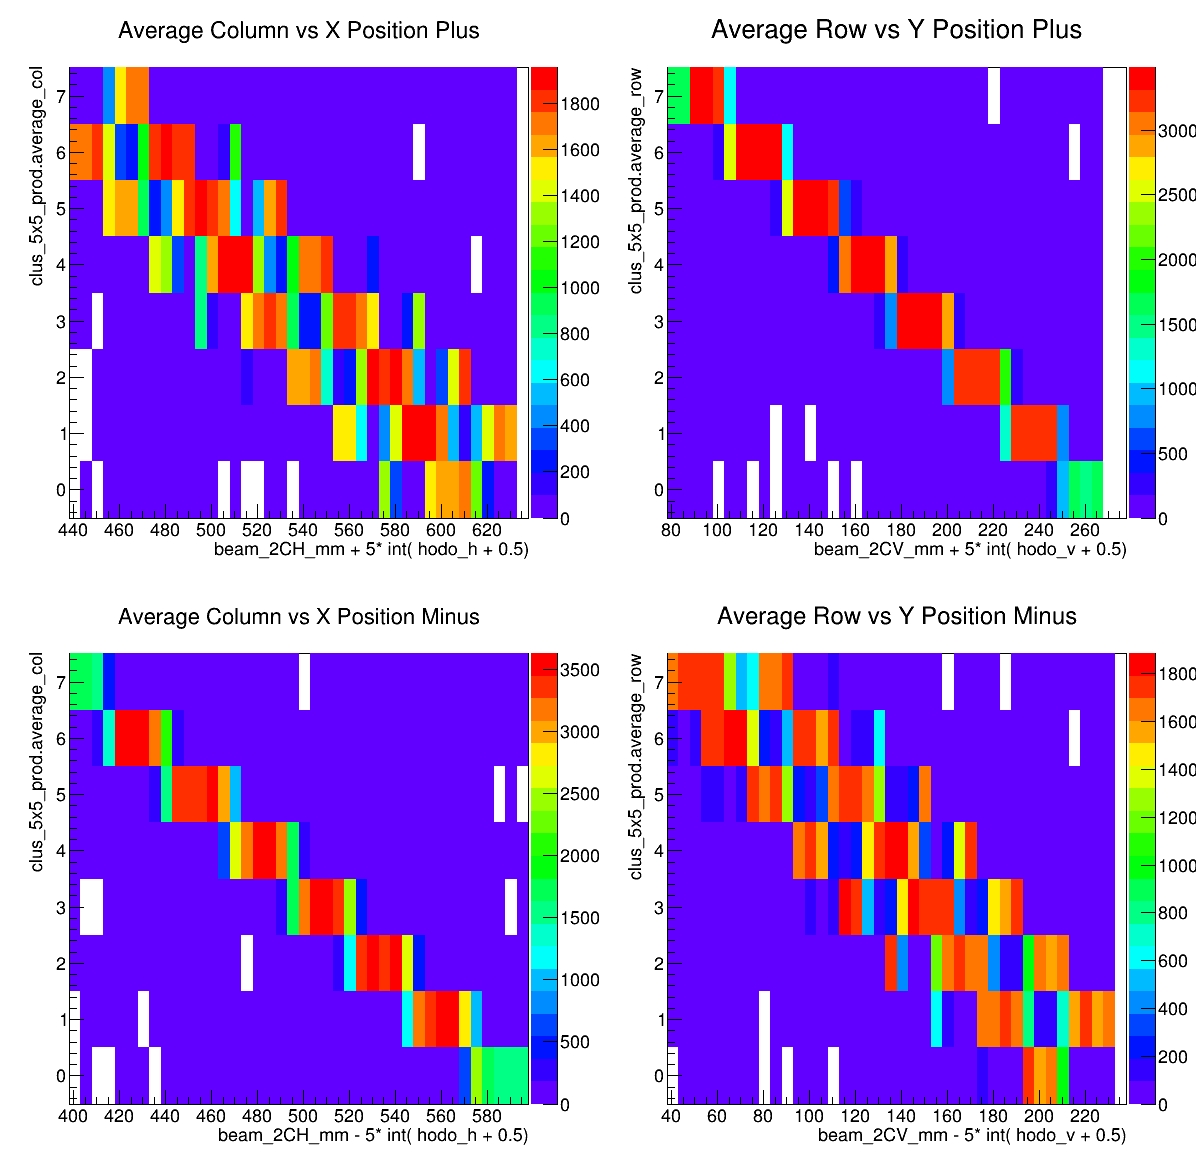
\includegraphics[width=0.38\textwidth]{Plots/Hodo/Hodoscope20183rd.png}
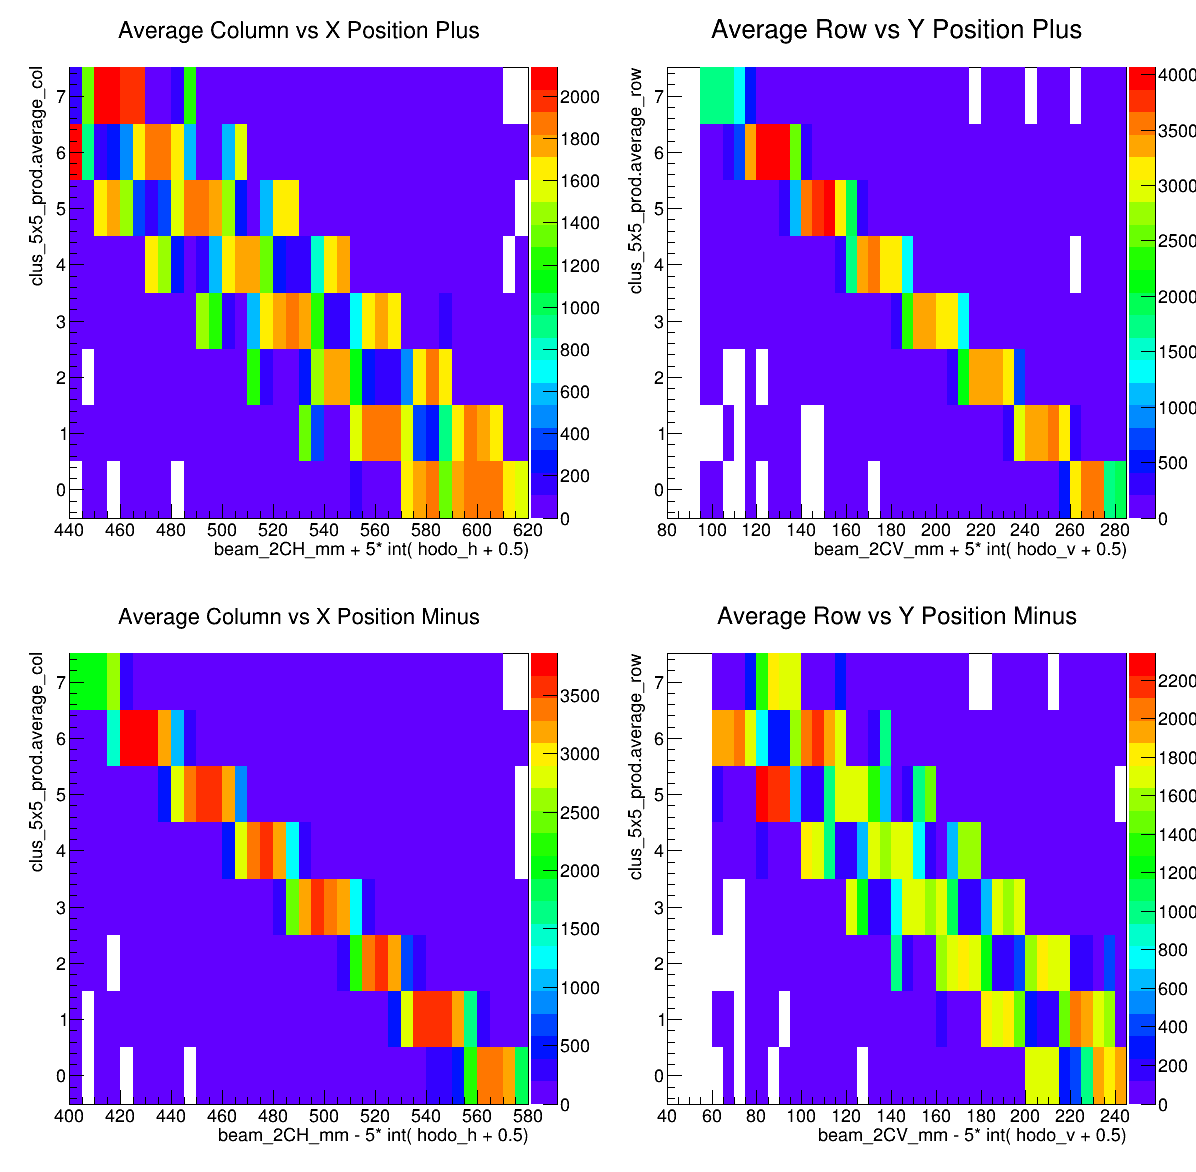
\includegraphics[width=0.38\textwidth]{Plots/Hodo/Hodoscope20184th.png}
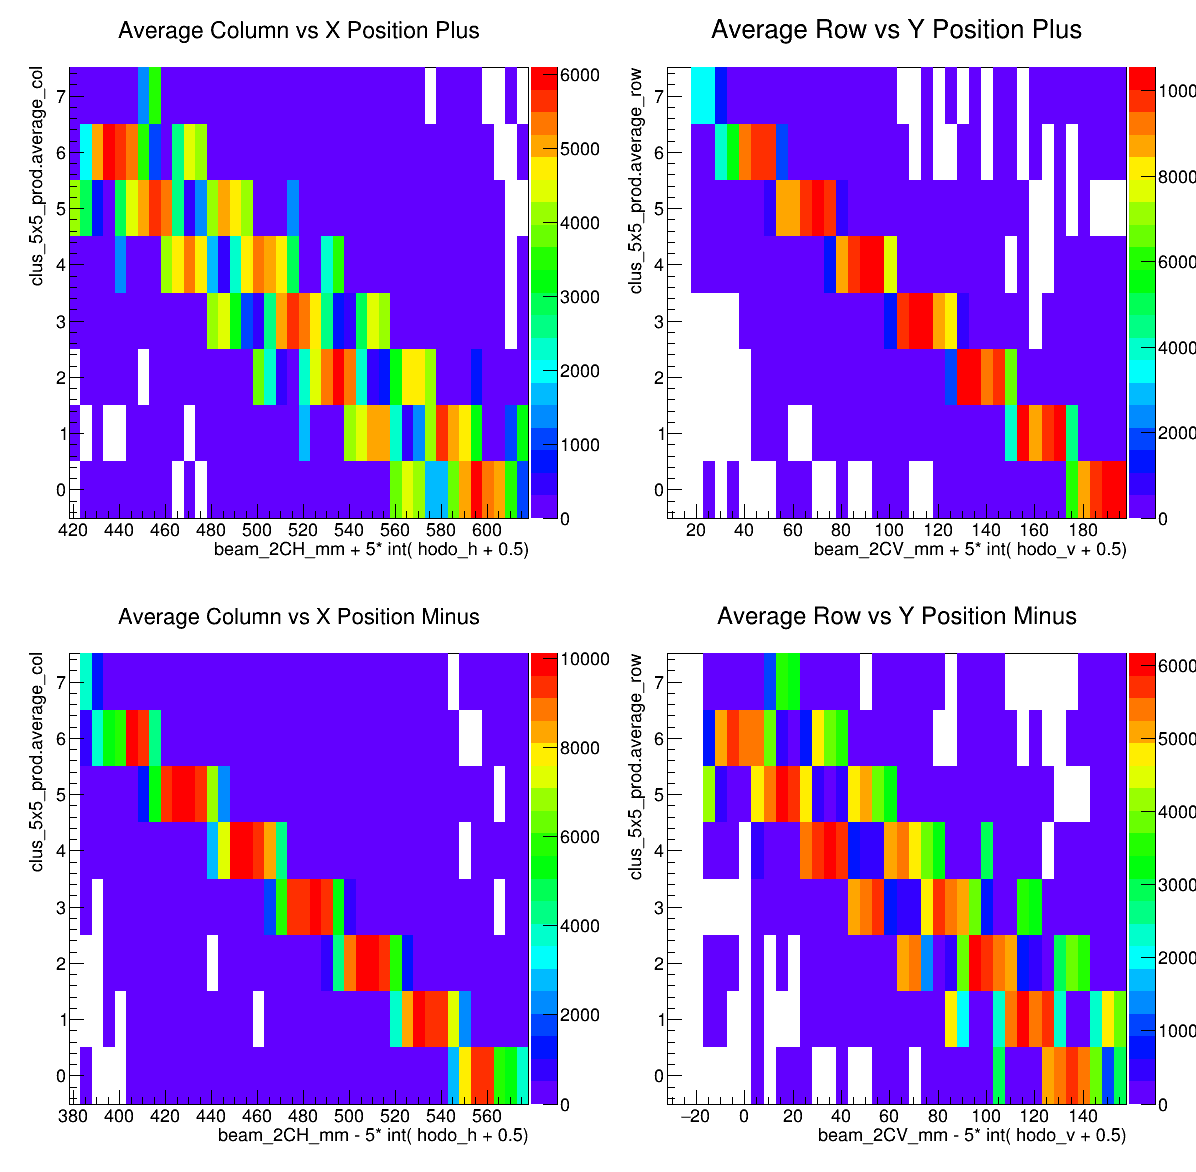
\includegraphics[width=0.30\textwidth]{Plots/Hodo/Hodoscope20185th.png}
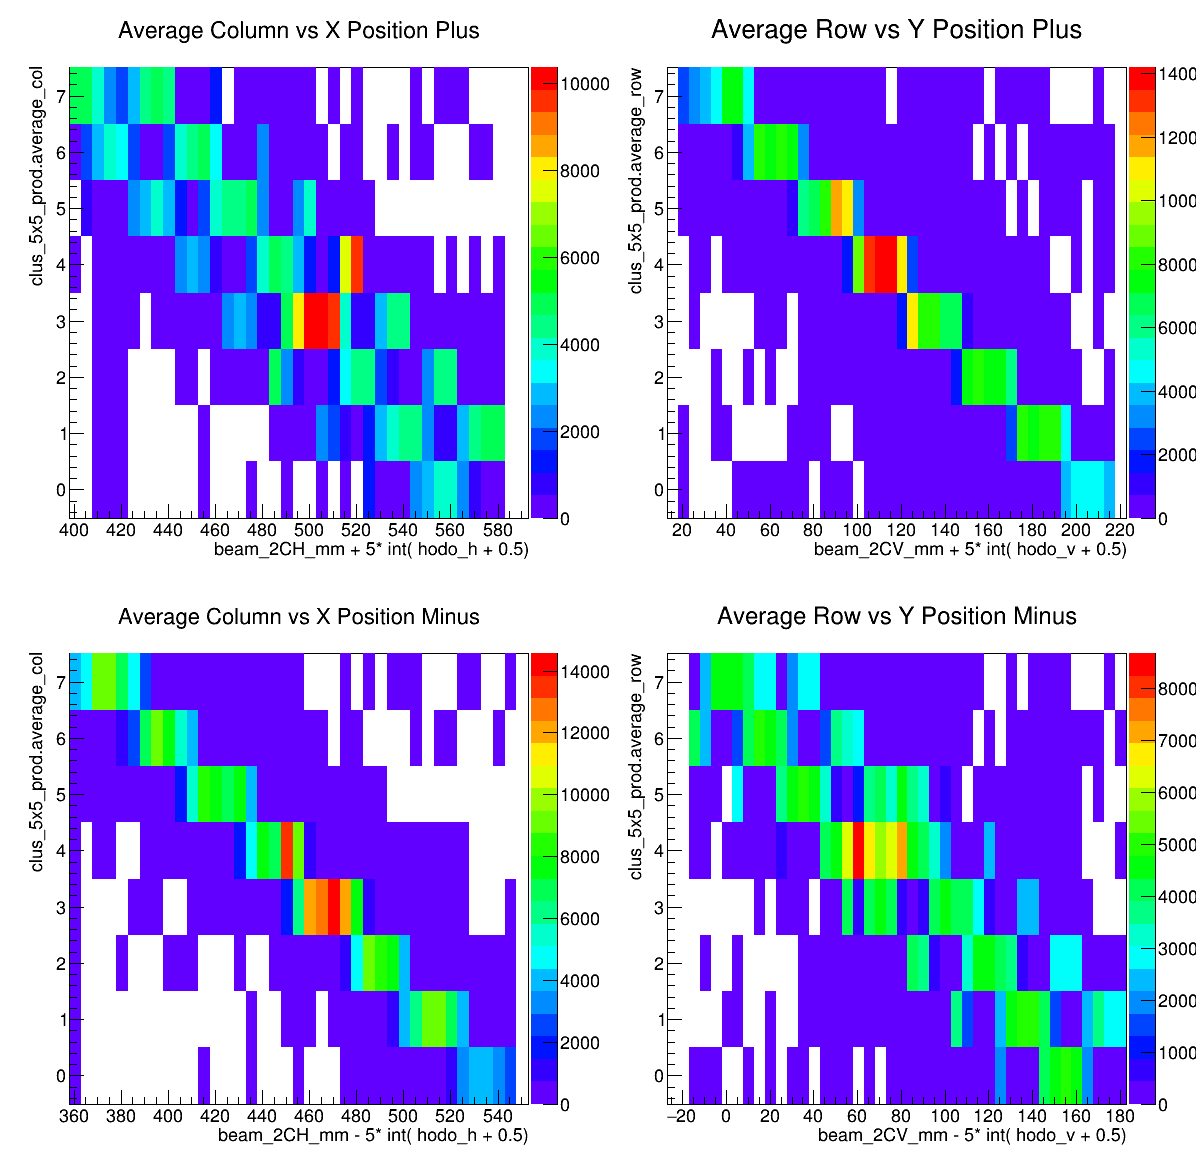
\includegraphics[width=0.30\textwidth]{Plots/Hodo/Hodoscope20186th.png}
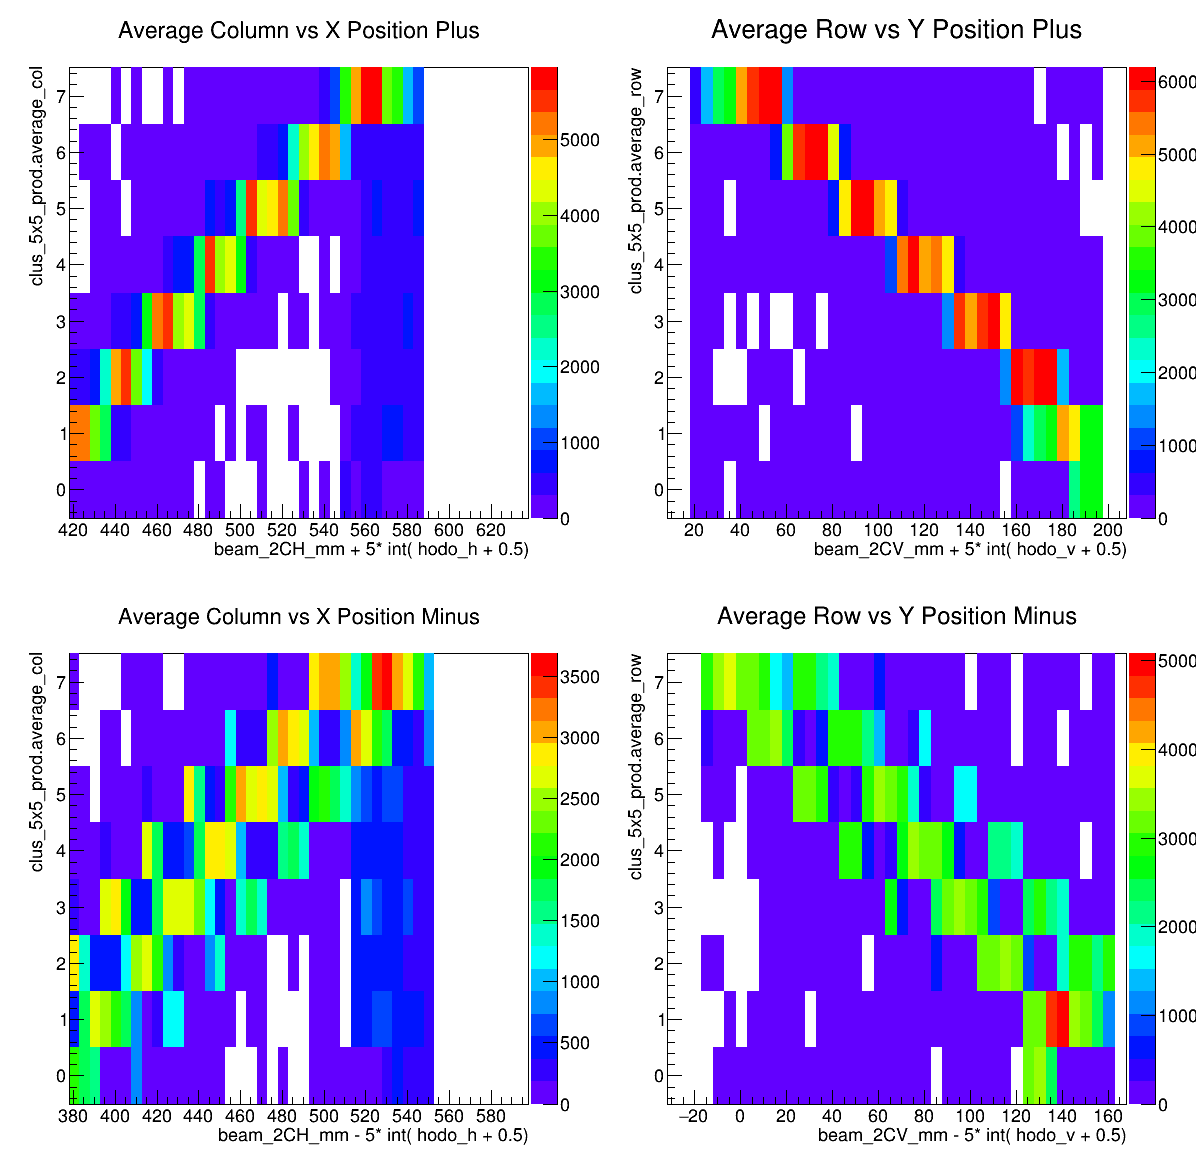
\includegraphics[width=0.30\textwidth]{Plots/Hodo/Hodoscope20187th.png}
\caption{The hodoscope corrections on the beam positions in the 2017 test beam second position scan ($10 \degree$ tilted, top left), third position scan ($0 \degree$ tilted, top right), 2018 test beam third position scan (dual channeling, middle left), fourth position scan (sPHENIX rotation to, middle right), fifth position scan (dual channeling, bottom left), sixth position scan (sPHENIX rotation + 5, bottom middle),  seventh position scan (sPHENIX rotation bottom right) on the EMCal with different signs are plotted above. We can see the ``-" sign for the horizontal position and "+" sign for the vertical direction give us step-like patterns for all plots except the seven position scan, which both  ``+" sign for horizontal and vertical scan actually give us the step-like pattern.}
\label{fig:hodoCorr}
\end{center}
\end{figure} 

\noindent Also, we are able to define the tower boundaries based on our hodoscope results shown on Figure~\ref{fig:hodoCorr}. The bound values are plotted into solid black lines in our next analyses to separate different towers.  

\subsection{Preliminary Data Assessment}

After correcting the position by the hodoscope, we are able to obtain the energy spectra vs the horizontal and vertical positions and make them into 3D histograms (TH3D). We apply ``good\_e" selections to the data. In the 2018 run, because of the delay of position recording, the position of the root file in our analysis is significantly different from the prdf file. It turns out that the prdf files have the correct positions. Therefore, we readout the prdf file and make a list to correct the position of the root file to the positions of prdf file. Table~\ref{tab:rootvsprdf} shows the difference between the horizontal and vertical positions of our analysis root files and the prdf files in the 4th position scan for a subset of runs (10 runs).

\begin{table}[h]
\centering
\begin{tabular}{|c|c|c|c|c|}
\hline
Run Number & prdf file x (mm)   &  prdf file y (mm) & root file x (mm)   &  root file y (mm)    \\
\hline
901  & 431.1  &  98.87 &    	431.1  &  98.9 \\
902  & 450.9  &  98.87 &	431  &  98.89 \\ 
903  & 471.1  &  98.87 &	450.9  &  98.87 \\ 
904  & 491.2  &  98.86 &			471.1  &  98.87 \\ 
905  & 510.9  &  98.9 &	491.2  &  98.86 \\ 
906  & 531  &  98.9 &	510.9  &  98.9 \\ 
907  & 551  &  98.89 &	531  &  98.9 \\ 
908  & 570.9  &  98.92 &	551  &  98.89 \\ 
909  & 0  &  98.93 &			570.9  &  98.92 \\ 
910  & 0  &  119 &			0  &  109.9 \\ 
\iffalse
911  & 0  &  0 &			0  &  0 \\ 
912  & 571  &  119 &			571  &  119 \\ 
913  & 551.1  &  119 &			571  &  119 \\ 
914  & 531.2  &  119 &			551  &  119 \\ 
915  & 511.1  &  119 &			531  &  119 \\ 
916  & 490.9  &  119 &			511  &  118.9 \\ 
917  & 0  &  0 &			0  &  0 \\ 
918  & 470.8  &  119 &			470.9  &  119 \\ 
919  & 451  &  119 &			451  &  119 \\ 
920  & 430.9  &  119 &			451  &  119 \\ 
921  & 0  &  0 &			0  &  0 \\ 
922  & 431.1  &  119 &			431.1  &  123.4 \\ 
923  & 431.1  &  139.1 &			431.1  &  133.6 \\ 
924  & 0  &  0 &			0  &  0 \\ 
925  & 0  &  0 &			0  &  0 \\ 
926  & 450.9  &  139.1 &			450.9  &  139.1 \\ 
927  & 471.1  &  139.1 &			451  &  139.1 \\ 
928  & 491.1  &  139.1 &			471.1  &  139.1 \\ 
929  & 511.2  &  139.1 &			491.1  &  139.1 \\ 
930  & 531  &  139.1 &			511.2  &  139.1 \\ 
931  & 551.1  &  139.1 &			531  &  139.1 \\ 
932  & 571.2  &  139.1 &			551  &  139.1 \\ 
933  & 0  &  139.1 &			571.1  &  139.1 \\ 
934  & 0  &  159 &			0  &  153 \\ 
935  & 571  &  159 &			0  &  159 \\ 
936  & 551.2  &  159 &			571  &  159 \\ 
937  & 531.1  &  159 &			551.1  &  159 \\ 
938  & 511.1  &  159 &			531.1  &  159 \\ 
939  & 490.9  &  159 &			511.2  &  159 \\ 
940  & 470.9  &  159 &			491  &  159 \\ 
\fi
\hline
\end{tabular}
\caption{Horizontal and vertical position prdf files and root files for 10 runs in the fourth position scan in the 2018 test beam run.}
\label{tab:rootvsprdf}
\end{table}

\noindent In the 3D histogram, we can see the energy spectrum of each position by doing a projection. In our 2017 analysis, we project the 3D histogram to a 1 mm $\times$ 1 mm square and study the energy spectrum because the beam spots for the position scans are not made to be uniformly spaced. In our 2018 analysis, since the beam spot are made to be uniform, we  project the 3D histogram to a 5 mm $\times$ 5 mm, which has more statistics and easier to put together to study the uniformity among different towers. Figure ~\ref{fig:Espect} shows the energy spectra of the second and third position scan in the 2017 test beam and third and fourth position scan in the 2018 test beam run. 



\begin{figure}[hbtp]
\begin{center}
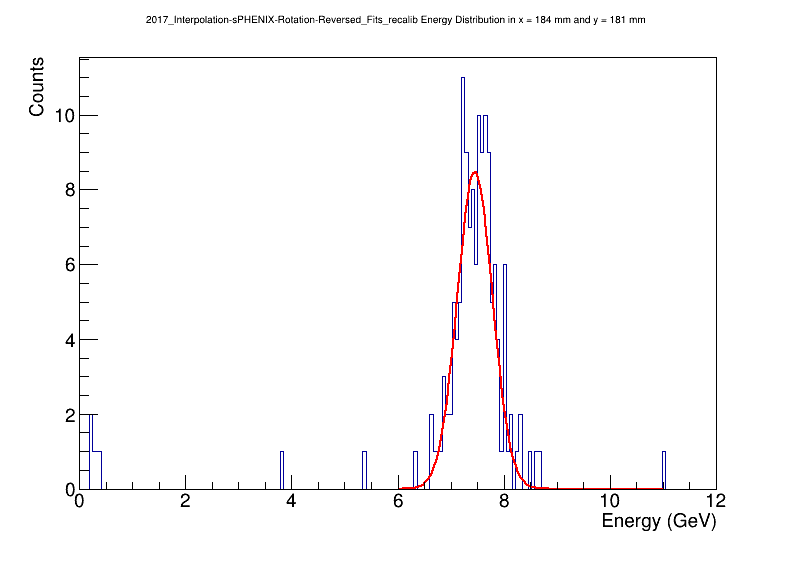
\includegraphics[width=0.38\textwidth]{Plots/Spectra/Plot_2017_Interpolation-sPHENIX-Rotation-Reversed_Fits_recalib_184-181.png}
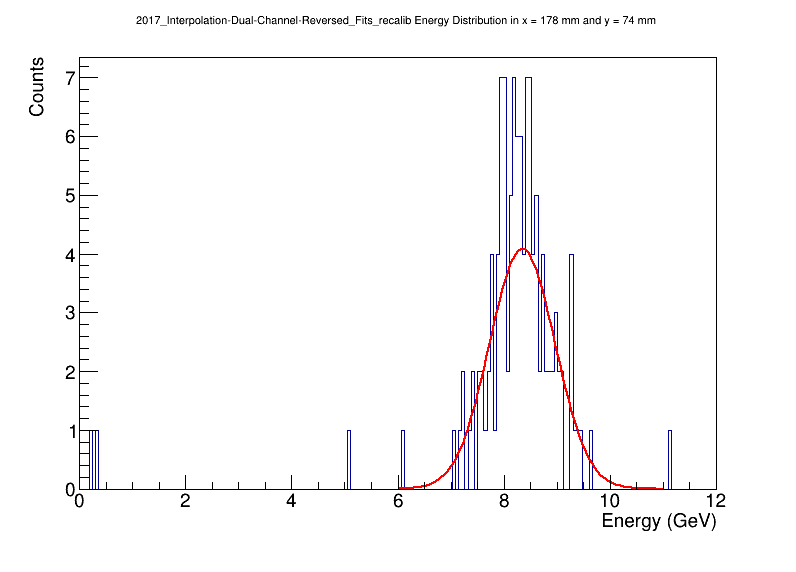
\includegraphics[width=0.38\textwidth]{Plots/Spectra/Plot_2017_Interpolation-Dual-Channel-Reversed_Fits_recalib_178-74.png}
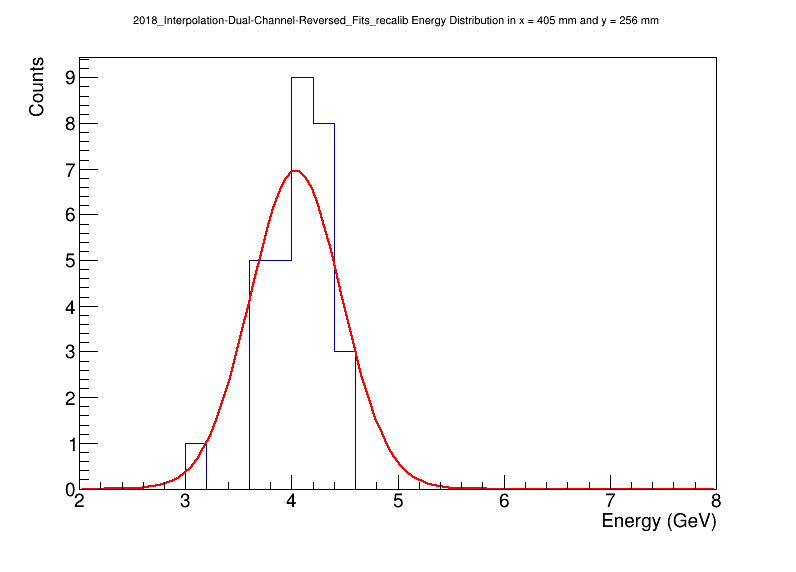
\includegraphics[width=0.38\textwidth]{Plots/Spectra/Plot_2018_Interpolation-Dual-Channel-Reversed_Fits_recalib_405-256.png}
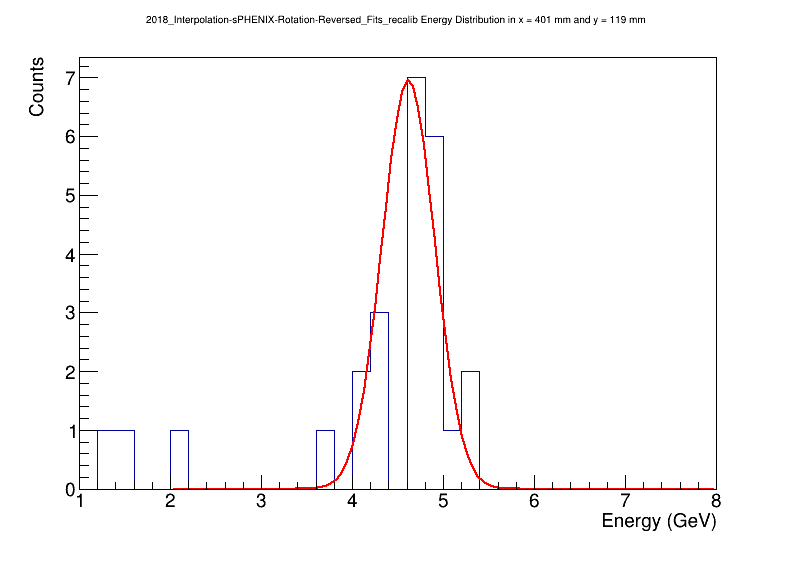
\includegraphics[width=0.38\textwidth]{Plots/Spectra/Plot_2018_Interpolation-sPHENIX-Rotation-Reversed_Fits_recalib_401-119.png}
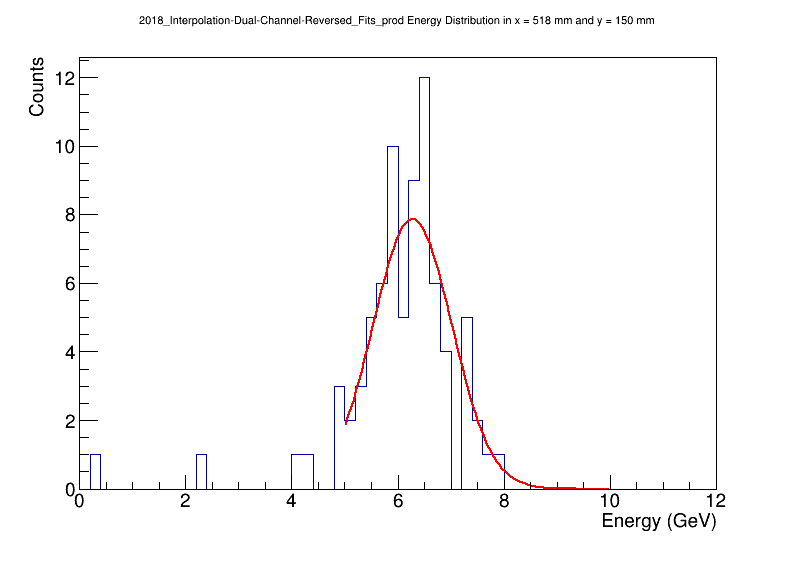
\includegraphics[width=0.38\textwidth]{Plots/Spectra/Plot_2018_Interpolation-Dual-Channel-Reversed_Fits_prod_518-150.png}
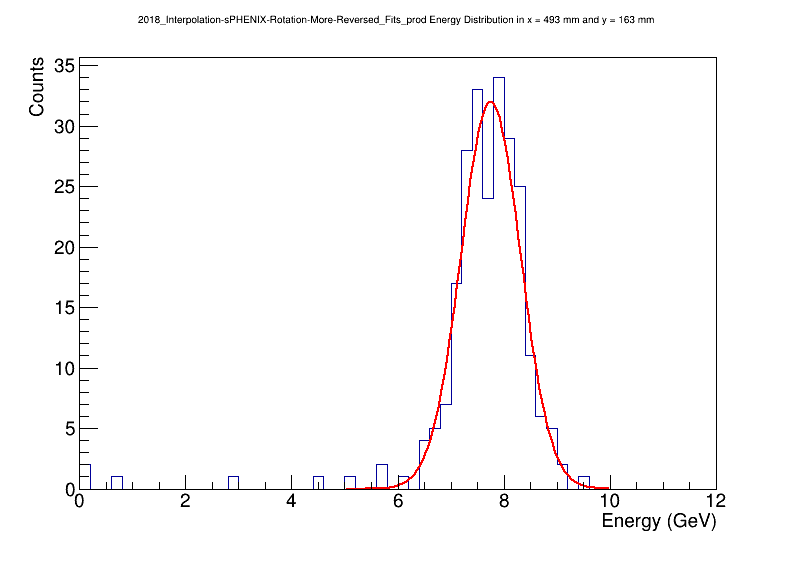
\includegraphics[width=0.38\textwidth]{Plots/Spectra/Plot_2018_Interpolation-sPHENIX-Rotation-More-Reversed_Fits_prod_493-163.png}
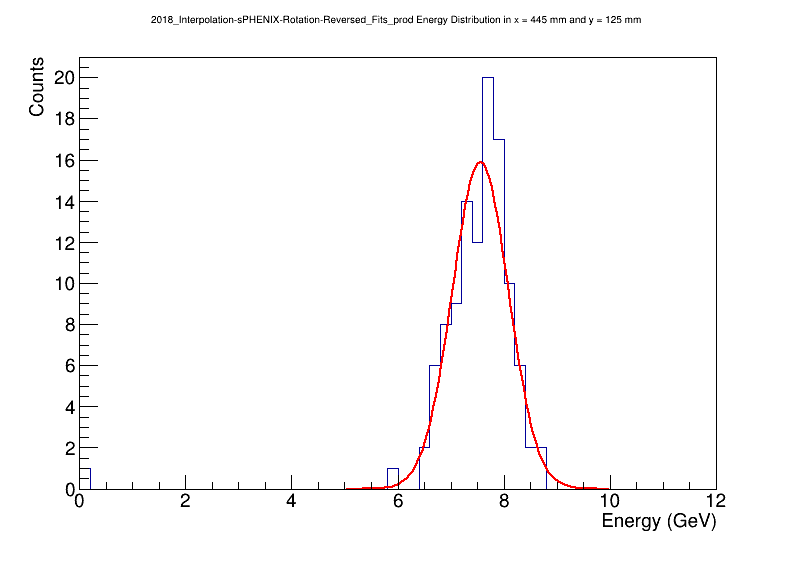
\includegraphics[width=0.38\textwidth]{Plots/Spectra/Plot_2018_Interpolation-sPHENIX-Rotation-Reversed_Fits_prod_445-125.png}
\caption{Energy spectra and Gaussian fits for the second scan (top left, x = 184 mm and y = 181 mm) and third position scan (top right, x = 178 mm and y = 74 mm) in the 2017 test beam run and the third position scan (middle left, x = 405 mm and y = 256 mm), the fourth position scan (middle right, x = 401 mm and y = 119mm), the fifth position scan (bottom left, x = 518 mm and y = 150 mm), the sixth position scan (bottom left, x = 493 mm and y = 163 mm), and the seventh position scan (bottom down, x = 445 mm and y = 125 mm) are shown above.}
\label{fig:Espect}
\end{center}
\end{figure} 

\noindent The statistics as a function of position are for the second and third position scan in 2017 test beam and third to seventh position scans in the 2018 test beam are shown in Figure ~\ref{fig:Stats}. 

\begin{figure}[hbtp]
\begin{center}
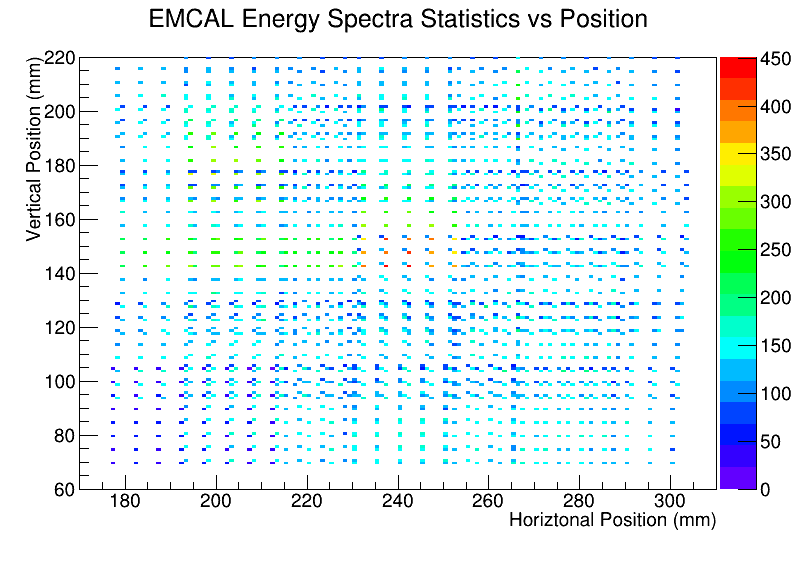
\includegraphics[width=0.38\textwidth]{Plots/StatPo/StatPo20172ndScan.png}
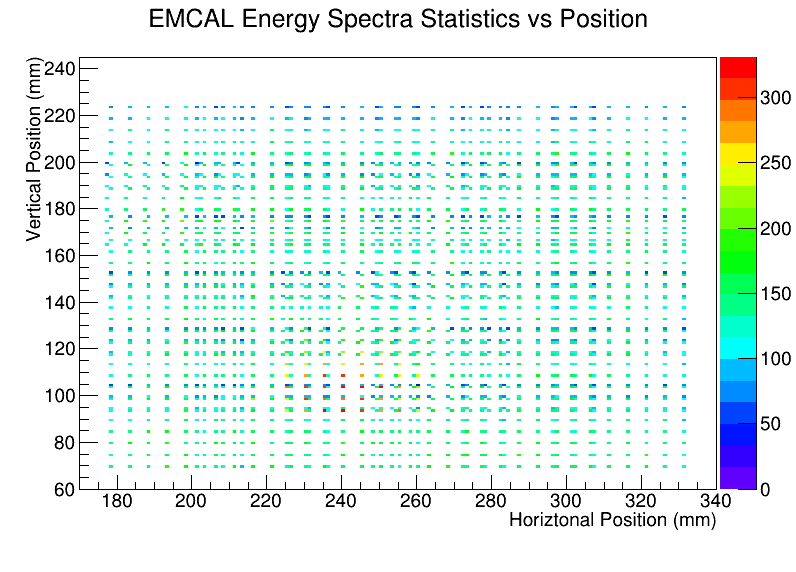
\includegraphics[width=0.38\textwidth]{Plots/StatPo/StatPo20173rdScan.png}
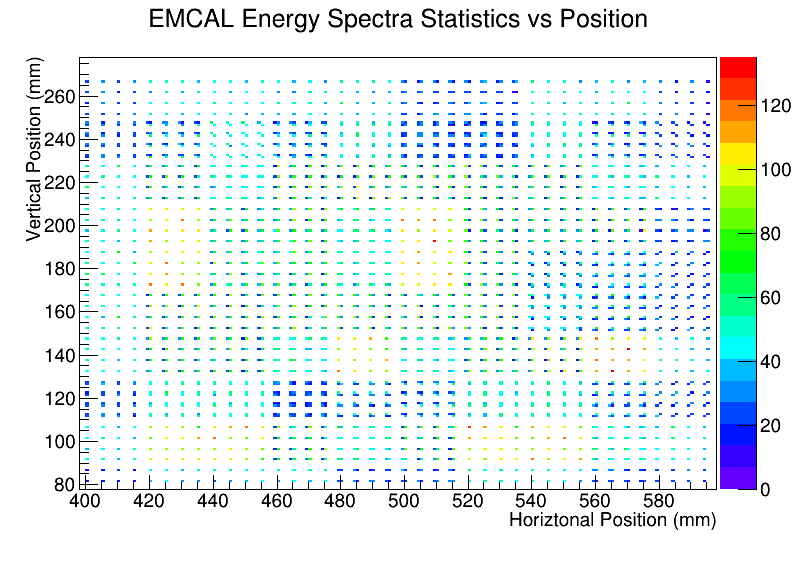
\includegraphics[width=0.38\textwidth]{Plots/StatPo/StatPo20183rdScan.png}
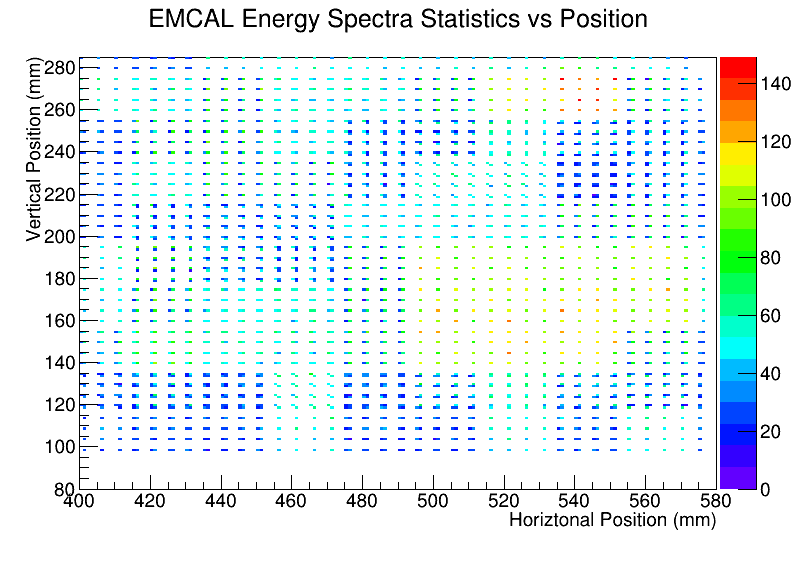
\includegraphics[width=0.38\textwidth]{Plots/StatPo/StatPo20184thScan.png}
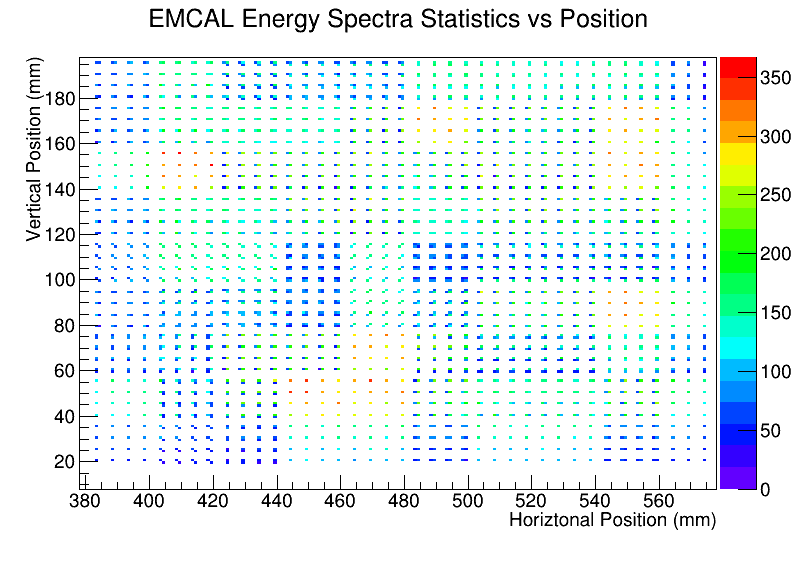
\includegraphics[width=0.38\textwidth]{Plots/StatPo/StatPo20185thScan.png}
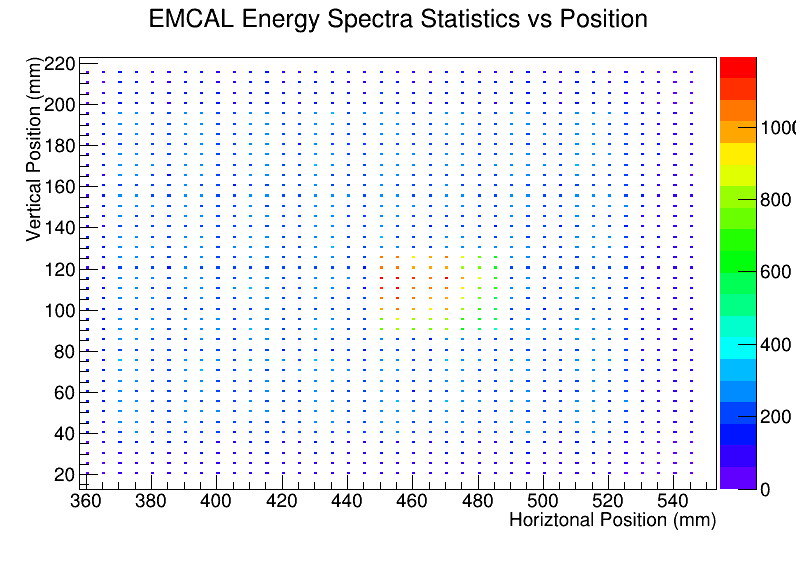
\includegraphics[width=0.38\textwidth]{Plots/StatPo/StatPo20186thScan.png}
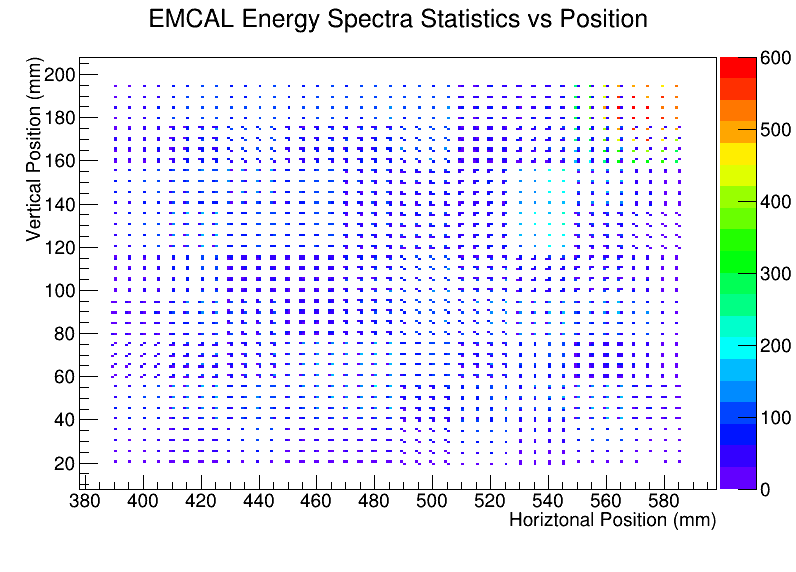
\includegraphics[width=0.38\textwidth]{Plots/StatPo/StatPo20187thScan.png}
\caption{The statistics vs the x-y position plots for the second and third position scans in the 2017 test beam run and the third to seventh position scans in the 2018 test beam run are shown from left to right and up to down respectfully above.}
\label{fig:Stats}
\end{center}
\end{figure} 

From Figure ~\ref{fig:Stats}, we can see that the 2017 test beam location non-uniformly scatters over the x-y plane while the 2018 test beam location has equal square-spacing in the x-y plane. Therefore, we need to do the interpolation to convert the 2017 position scan make the mean energy vs position continuous analysis and can directly use the result from 2018 test beam for the mean energy vs position plots.

\subsection{Mean Energy Values Extraction}

To extract the energy spectrum, we use two different methods: mean value and Gaussian fits. For the mean method, we define the energy range in each scan and then just take the mean of the spectrum. For the Gaussian Fits method, we define the energy range of the histogram, fit range, and the correction range for failed fits. Basically, we fit the energy spectrum with a Gaussian within a reasonable range where the peak of the Gaussian is contained. If our fits fails, we should get some mean values from the fit that greatly deviate from our expectation. Therefore, for the failed fits, we will replace the fits means by the just a mean from the distribution. Both methods have their own advantages: the mean method is good when the statistics of the energy spectra are low while the fits method effective reduces the contribution of outlier when we extract the mean from the energy spectra. Therefore, for each position bin, we have one mean energy value. The mean energy vs position for the mean results for the second and third position scan in the 2017 test beam and third to seventh scan in the 2018 test beam with mean method are shown in Figure~\ref{fig:MeanMethod} and fits method are shown Figure~\ref{fig:FitsMethod}. 

\begin{figure}[hbtp]
\begin{center}
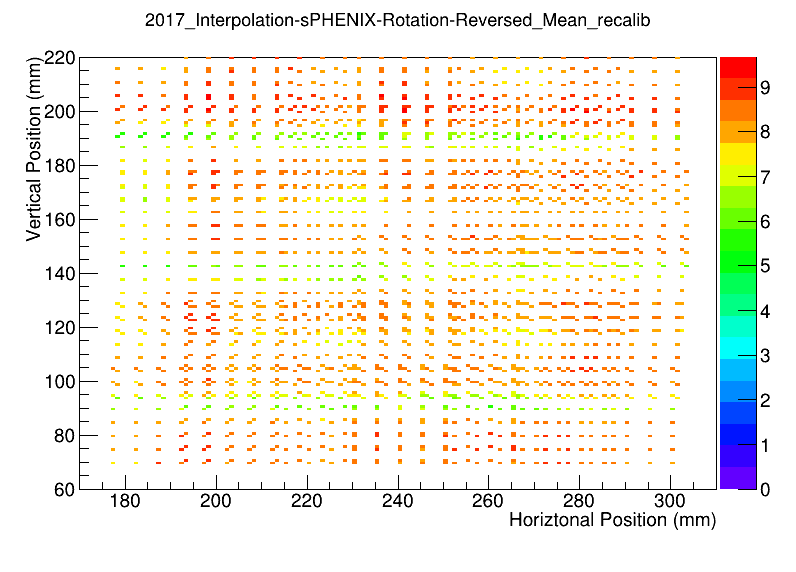
\includegraphics[width=0.38\textwidth]{Plots/EnpoMeanMethod/EnPo20172ndScan.png}
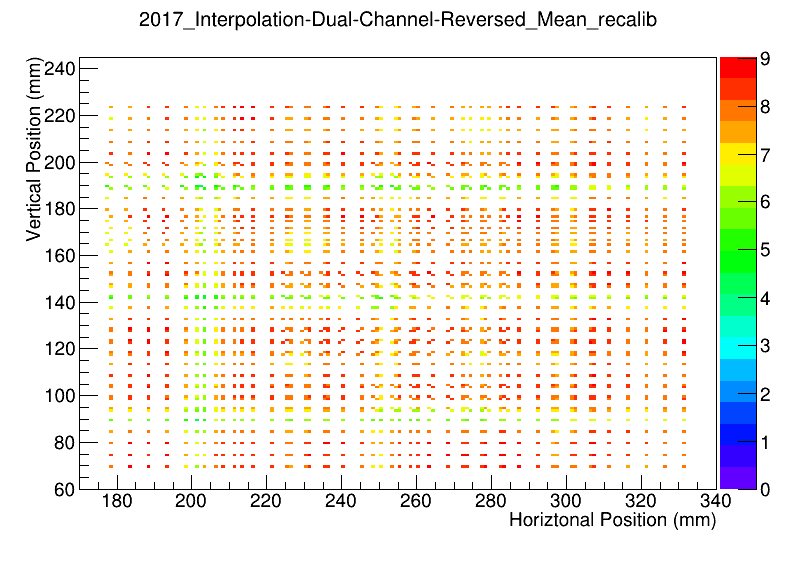
\includegraphics[width=0.38\textwidth]{Plots/EnpoMeanMethod/EnPo20173rdScan.png}
\includegraphics[width=0.38\textwidth]{Plots/EnpoMeanMethod/EnPo20183rdScan.png}
\includegraphics[width=0.38\textwidth]{Plots/EnpoMeanMethod/EnPo20184thScan.png}
\includegraphics[width=0.33\textwidth]{Plots/EnpoMeanMethod/EnPo20185thScan.png}
\includegraphics[width=0.33\textwidth]{Plots/EnpoMeanMethod/EnPo20186thScan.png}
\includegraphics[width=0.33\textwidth]{Plots/EnpoMeanMethod/EnPo20187thScan.png}
\caption{The mean energy vs position with the mean method in the 2017 test beam (binning 1 mm $\times$ 1 mm) second position scan ($10 \degree$ tilted, top left), third position scan ($0 \degree$ tilted, top right), 2018 test beam (binning 1 mm $\times$ 1 mm)  third position scan (dual channeling, middle left), fourth position scan (sPHENIX rotation to, middle right), fifth position scan (dual channeling, bottom left), sixth position scan (sPHENIX rotation + 5, bottom middle),  seventh position scan (sPHENIX rotation bottom right) on the EMCal are plotted above.}
\label{fig:MeanMethod}
\end{center}
\end{figure} 


\begin{figure}[hbtp]
\begin{center}
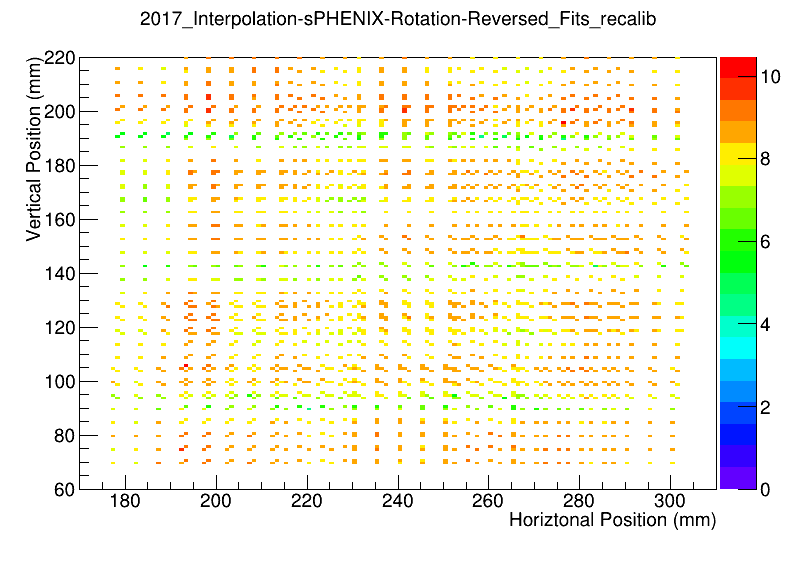
\includegraphics[width=0.38\textwidth]{Plots/EnpoFitsMethod/EnPo20172ndScan.png}
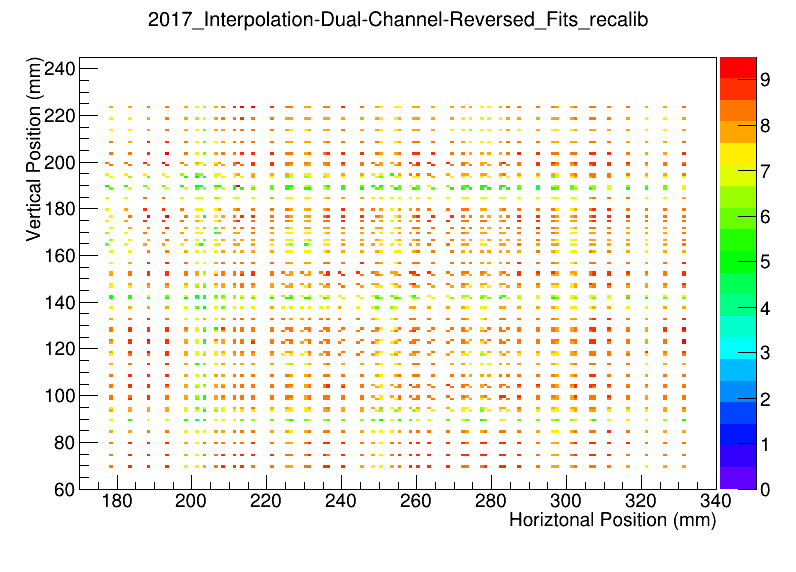
\includegraphics[width=0.38\textwidth]{Plots/EnpoFitsMethod/EnPo20173rdScan.png}
\includegraphics[width=0.38\textwidth]{Plots/EnpoFitsMethod/EnPo20183rdScan.png}
\includegraphics[width=0.38\textwidth]{Plots/EnpoFitsMethod/EnPo20184thScan.png}
\includegraphics[width=0.33\textwidth]{Plots/EnpoFitsMethod/EnPo20185thScan.png}
\includegraphics[width=0.33\textwidth]{Plots/EnpoFitsMethod/EnPo20186thScan.png}
\includegraphics[width=0.33\textwidth]{Plots/EnpoFitsMethod/EnPo20187thScan.png}
\caption{The mean energy vs position with the fits method in the 2017 test beam (binning 1 mm $\times$ 1 mm) second position scan ($10 \degree$ tilted, top left), third position scan ($0 \degree$ tilted, top right), 2018 test beam (binning 1 mm $\times$ 1 mm)  third position scan (dual channeling, middle left), fourth position scan (sPHENIX rotation to, middle right), fifth position scan (dual channeling, bottom left), sixth position scan (sPHENIX rotation + 5, bottom middle),  seventh position scan (sPHENIX rotation bottom right) on the EMCal with different signs are plotted above.}
\label{fig:FitsMethod}
\end{center}
\end{figure} 

As we can see from Figure~\ref{fig:FitsMethods}, the position for the 2018 test beam is uniformly distributed while the 2017 test beam is not. Therefore, for the 2018 test beam results, we can just expand each 1 mm $\times$ 1 mm spots to a continuous 5 mm $\times$ 5 mm spots. For the 2017 test beam results, we need to perform interpolation to obtain the mean energy values for the white spots to make the energy vs x-y position plots continuous. 

\subsection{Interpolation and Reversion}

\noindent With the input from the mean energy vs position plots above in the previous section, we are able to perform interpolation. The interpolation code is based on the simple linear interpolation algorithm. We define a rectangular $(\pm x) \times (\pm y)$ scan to include all none zero value near the empty bin and then take the unweighted average of all non-zero values. In our analysis, we choose $(\pm 2)$ mm $ \times (\pm 2)$ mm scan steps and basically we get one value in each of the four directions. In addition to interpolation, we need to reverse the x and y axis because of the positions of the towers in the test beam, which face up, are exactly opposite to what it is measure, which face down. Figure~\ref{fig:MeanMethods} and Figure~\ref{fig:FitsMethods} display our interpolation with mean and Gaussian Fits method + reversion results for the 2017 test beam and the 2018 test beam (not necessary to perform interpolation due to its uniformity):

\begin{figure}[hbtp]
\begin{center}
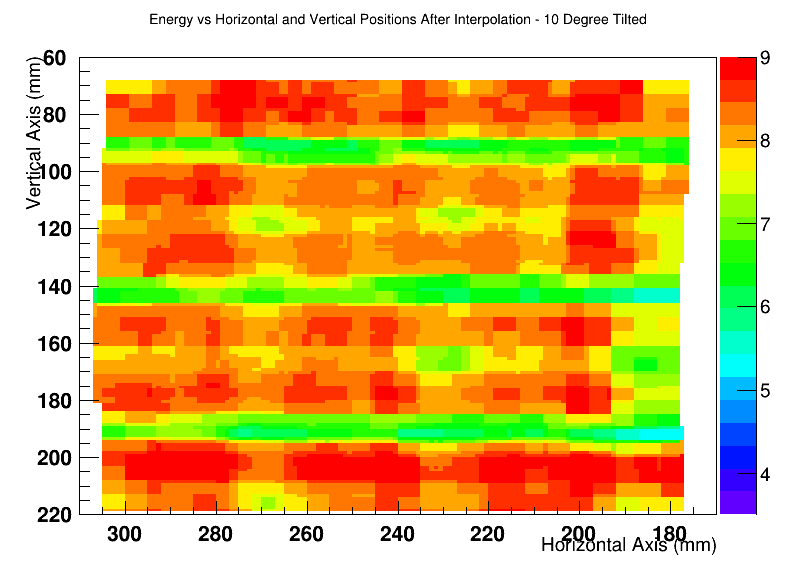
\includegraphics[width=0.38\textwidth]{Plots/InterMean/Inter20172ndScan.png}
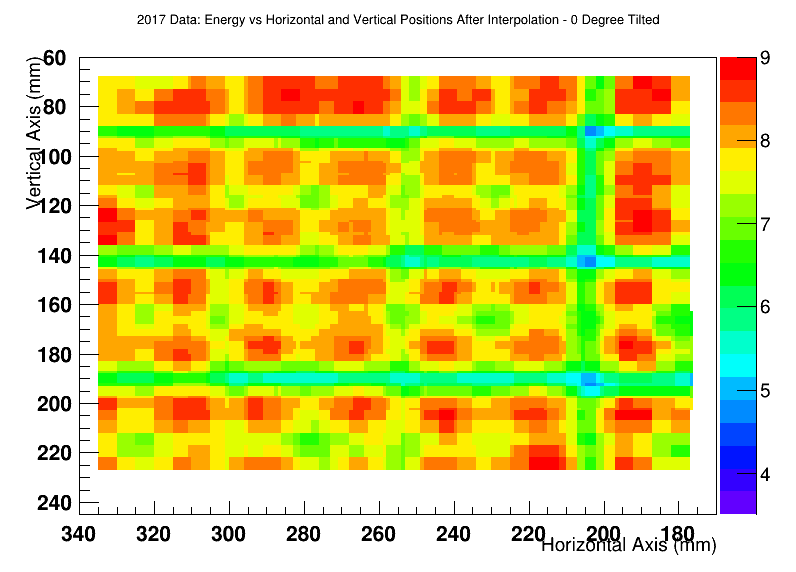
\includegraphics[width=0.38\textwidth]{Plots/InterMean/Inter20173rdScan.png}
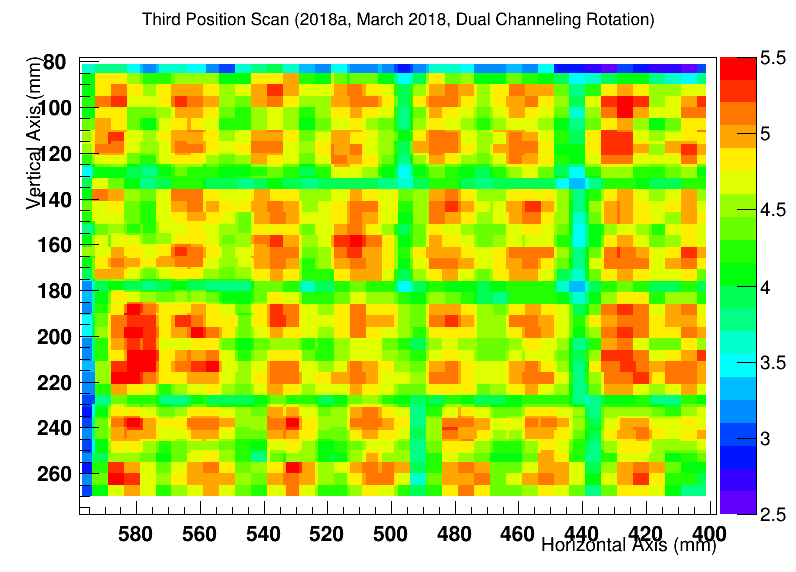
\includegraphics[width=0.38\textwidth]{Plots/InterMean/Inter20183rdScan.png}
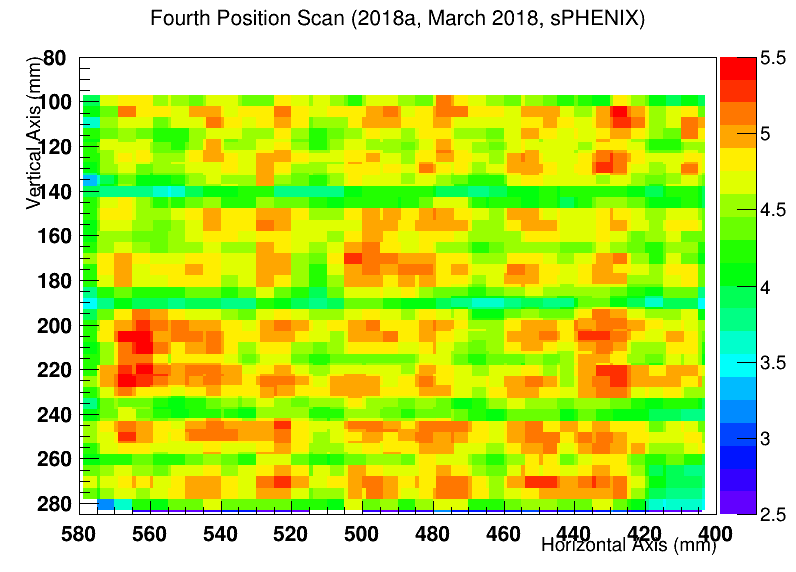
\includegraphics[width=0.38\textwidth]{Plots/InterMean/Inter20184thScan.png}
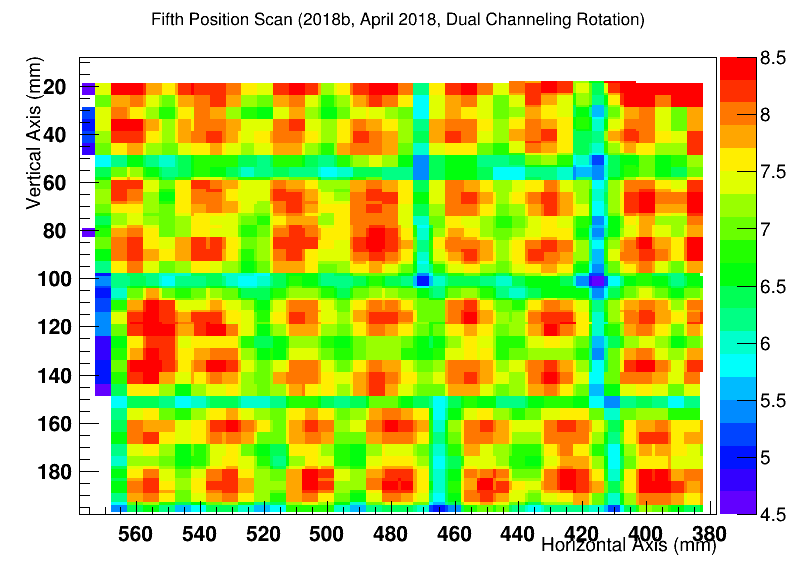
\includegraphics[width=0.38\textwidth]{Plots/InterMean/Inter20185thScan.png}
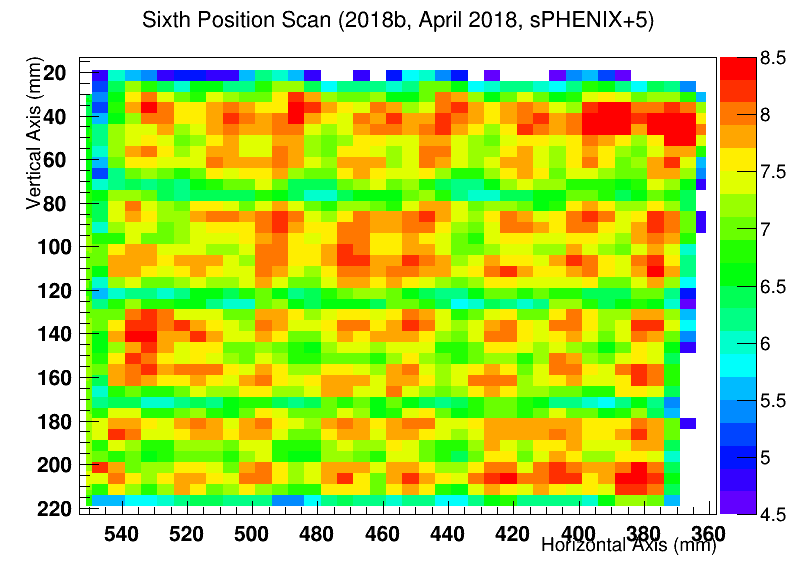
\includegraphics[width=0.38\textwidth]{Plots/InterMean/Inter20186thScan.png}
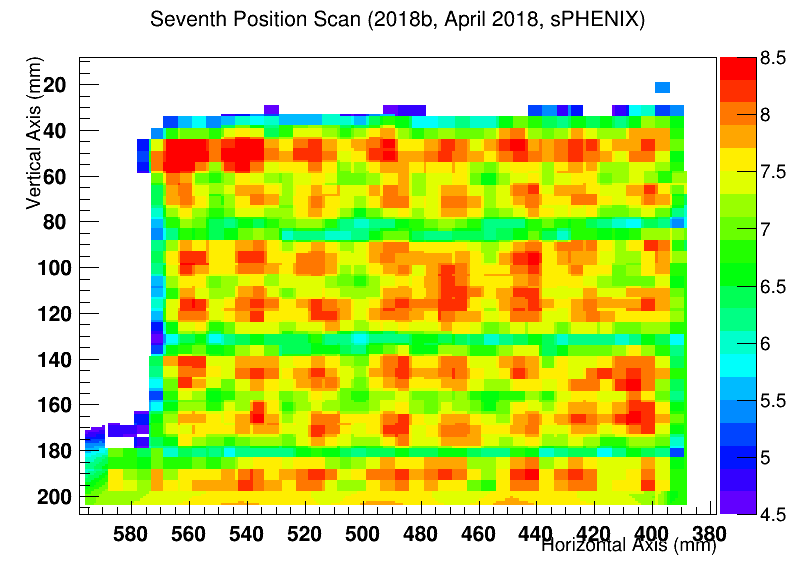
\includegraphics[width=0.38\textwidth]{Plots/InterMean/Inter20187thScan.png}
\caption{The interpolated mean energy vs position with the mean method in the 2017 test beam second position scan ($10 \degree$ tilted, top left), third position scan ($0 \degree$ tilted, top right), 2018 test beam third position scan (dual channeling, middle left), fourth position scan (sPHENIX rotation to, middle right), fifth position scan (dual channeling, bottom left), sixth position scan (sPHENIX rotation + 5, bottom middle),  seventh position scan (sPHENIX rotation bottom right) on the EMCal with different signs are plotted above.}
\label{fig:MeanMethods}
\end{center}
\end{figure} 

\begin{figure}[hbtp]
\begin{center}
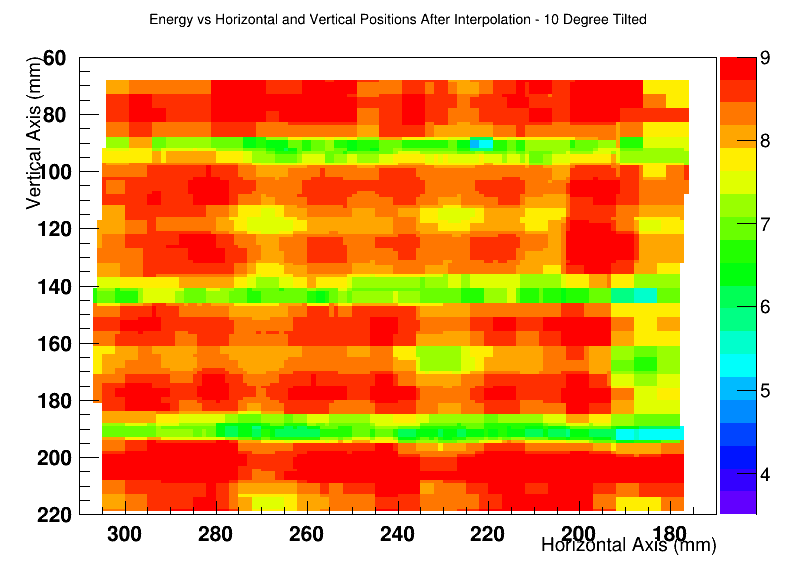
\includegraphics[width=0.38\textwidth]{Plots/InterFits/Inter20172ndScan.png}
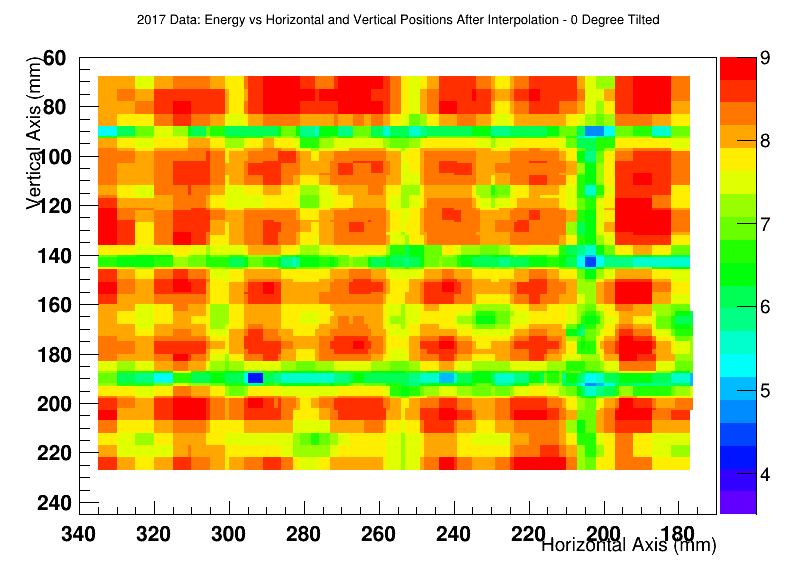
\includegraphics[width=0.38\textwidth]{Plots/InterFits/Inter20173rdScan.png}
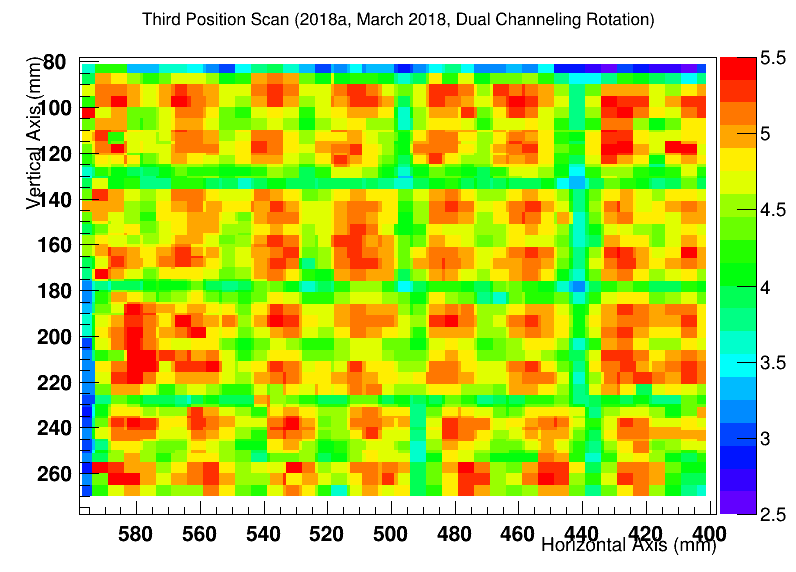
\includegraphics[width=0.38\textwidth]{Plots/InterFits/Inter20183rdScan.png}
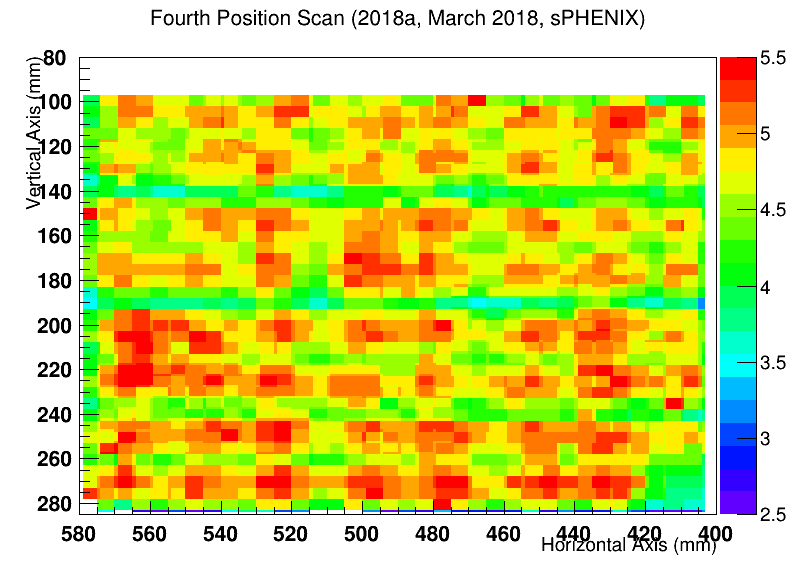
\includegraphics[width=0.38\textwidth]{Plots/InterFits/Inter20184thScan.png}
\includegraphics[width=0.38\textwidth]{Plots/InterFits/Inter20185thScan.png}
\includegraphics[width=0.38\textwidth]{Plots/InterFits/Inter20186thScan.png}
\includegraphics[width=0.38\textwidth]{Plots/InterFits/Inter20187thScan.png}
\caption{The interpolated mean energy vs position with the fits method in the 2017 test beam second position scan ($10 \degree$ tilted, top left), third position scan ($0 \degree$ tilted, top right), 2018 test beam third position scan (dual channeling, middle left), fourth position scan (sPHENIX rotation to, middle right), fifth position scan (dual channeling, bottom left), sixth position scan (sPHENIX rotation + 5, bottom middle),  seventh position scan (sPHENIX rotation bottom right) on the EMCal with different signs are plotted above.}
\label{fig:FitsMethods}
\end{center}
\end{figure} 

\subsection{Tower Boundaries Implementation}

Finally, we implement the tower boundaries to our interpolated (continuous) energy vs position plots according to the steps in the hodoscope correction plots. Also, we remove the interpolation for the 2018 test beam results because of the uniform spacing. Figure~\ref{fig:BlockEMCAL} shows the Second position scan in the 2017 test beam and the corresponding the EMCal block configuration. 

\begin{figure}[hbtp]
\begin{center}
\includegraphics[width=0.38\textwidth]{Plots/BlockConfig/Inter20172ndScanLabeled.png}
\includegraphics[width=0.38\textwidth]{Plots/BlockConfig/Inter20173rdScanLabeled.png}
\includegraphics[width=0.38\textwidth]{Plots/BlockConfig/BlockConfig.png}
\caption{The interpolated mean energy vs position with the fits method in the 2017 test beam second position scan with EMCal boundaries ($10 \degree$ tilted, top left), third position scan ($0 \degree$ tilted, top right), and the corresponding EMCal block configuration (down middle) are shown above.}
\label{fig:BlockEMCAL}
\end{center}
\end{figure} 

The energy vs position plots for mean and fit for the  2017 test beam run with tower boundaries are show on Fig~\ref{fig:MeanWithLineMethods} and Fig~\ref{fig:FitsWithLineMethods} respectfully. 


\begin{figure}[hbtp]
\begin{center}
\includegraphics[width=0.38\textwidth]{Plots/InterMeanWithLine/Inter20172ndScan.png}
\includegraphics[width=0.38\textwidth]{Plots/InterMeanWithLine/Inter20173rdScan.png}
\includegraphics[width=0.38\textwidth]{Plots/2018NoInterMean/EnPo20183rdScan.png}
\includegraphics[width=0.38\textwidth]{Plots/2018NoInterMean/EnPo20184thScan.png}
\includegraphics[width=0.38\textwidth]{Plots/2018NoInterMean/EnPo20185thScan.png}
\includegraphics[width=0.38\textwidth]{Plots/2018NoInterMean/EnPo20186thScan.png}
\includegraphics[width=0.38\textwidth]{Plots/2018NoInterMean/EnPo20187thScan.png}
\caption{The interpolated mean energy vs position with the mean method in the 2017 test beam second position scan ($10 \degree$ tilted, top left), third position scan ($0 \degree$ tilted, top right), 2018 test beam third position scan (dual channeling, middle left), fourth position scan (sPHENIX rotation to, middle right), fifth position scan (dual channeling, bottom left), sixth position scan (sPHENIX rotation + 5, bottom middle),  seventh position scan (sPHENIX rotation bottom right) on the EMCal are plotted above.}
\label{fig:MeanWithLineMethods}
\end{center}
\end{figure} 


\begin{figure}[hbtp]
\begin{center}
\includegraphics[width=0.38\textwidth]{Plots/InterFitsWithLine/Inter20172ndScan.png}
\includegraphics[width=0.38\textwidth]{Plots/InterFitsWithLine/Inter20173rdScan.png}
\includegraphics[width=0.38\textwidth]{Plots/2018NoInterFits/EnPo20183rdScan.png}
\includegraphics[width=0.38\textwidth]{Plots/2018NoInterFits/EnPo20184thScan.png}
\includegraphics[width=0.38\textwidth]{Plots/2018NoInterFits/EnPo20185thScan.png}
\includegraphics[width=0.38\textwidth]{Plots/2018NoInterFits/EnPo20186thScan.png}
\includegraphics[width=0.38\textwidth]{Plots/2018NoInterFits/EnPo20187thScan.png}
\caption{The interpolated mean energy vs position with the fits method in the 2017 test beam second position scan ($10 \degree$ tilted, top left), third position scan ($0 \degree$ tilted, top right), 2018 test beam third position scan (dual channeling, middle left), fourth position scan (sPHENIX rotation to, middle right), fifth position scan (dual channeling, bottom left), sixth position scan (sPHENIX rotation + 5, bottom middle),  seventh position scan (sPHENIX rotation bottom right) on the EMCa are plotted above.}
\label{fig:FitsWithLineMethods}
\end{center}
\end{figure} 

As we can see, the mean energy vs position results are consistent with the boundaries from hodoscope corrections and the block configuration for the EMCal prototypes. The centers of the towers have higher average energy close to the beam energy. The boundaries has lower energy that the centers due to loss in electromagnetic shower collection, which contributes to the non-uniformity of the EMCal. From now on, we will conduct further analysis on fits method only because we have enough statistics to perform reasonable Gaussian fits. Fits method will reduce the bias of the outliers in the energy spectra when we extract the mean.


\section{Further Analysis}

\subsection{1D Projections and Comparisons}

Our analysis results from Figure~\ref{fig:MeanWithLineMethods}, Figure~\ref{fig:FitsWithLineMethods} are intuitive because it provides big pictures of the EMCal performance. However, it only provides us qualitative understandings of the EMCal uniformity. To better study the EMCal performance, we need to perform 1D projections to analyze our data quantitatively and compare the 2017 test beam results with the 2018 test beam results to see if we have improved our EMCal prototypes. Therefore, we horizontally and vertically project the energy vs position plots on the centers of the towers and the boundaries of the towers to quantitative analyze the non-uniformity of EMCal. Figure~\ref{fig:1DProjCenH2017}, Figure~\ref{fig:1DProjCenV2017}, Figure~\ref{fig:1DProjCenH2018} and Figure~\ref{fig:1DProjCenV2018} respectfully show the 1D horizontal and vertical projections (normalized by the average value of the central 2 $\times$ 2 towers shown on Figure~\ref{fig:TowerNormj}) on the horizontal direction in the centers and the boundaries of the towers in the second and third position scans in 2017 test beam run and third to seventh position scan in the 2018 test beam run. 

\begin{figure}[hbtp]
\begin{center}
\includegraphics[width=0.45\textwidth]{Plots/2017/2nd/Normalized.png}
\includegraphics[width=0.45\textwidth]{Plots/2017/3rd/Normalized.png}
\includegraphics[width=0.45\textwidth]{Plots/2018/3rd/Normalized.png}
\includegraphics[width=0.45\textwidth]{Plots/2018/4th/Normalized.png}
\includegraphics[width=0.45\textwidth]{Plots/2018/5th/Normalized.png}
\includegraphics[width=0.45\textwidth]{Plots/2018/6th/Normalized.png}
\includegraphics[width=0.45\textwidth]{Plots/2018/7th/Normalized.png}
\caption{The normalization region of the central 2 $\times$ 2 towers of the second and third position scan in the 2017 test beam run and the third to seventh scan in the 2018 test beam run are show from left to right and up to down above.}
\label{fig:TowerNormj}
\end{center}
\end{figure} 

\begin{figure}[hbtp]
\begin{center}
\includegraphics[width=0.45\textwidth]{Plots/2017/2nd/CombY5.png}
\includegraphics[width=0.45\textwidth]{Plots/2017/2nd/CombY6.png}
\includegraphics[width=0.45\textwidth]{Plots/2017/3rd/CombY5.png}
\includegraphics[width=0.45\textwidth]{Plots/2017/3rd/CombY6.png}
\caption{The horizontal projections on the centers of the towers (left) and boundaries of the towers(right) of mean energy vs position with the fits method in the 2017 test beam second position scan ($10 \degree$ tilted, first row) and third position scan ($0 \degree$ tilted, second row) on the EMCal are show above}
\label{fig:1DProjCenH2017}
\end{center}
\end{figure} 

\begin{figure}[hbtp]
\begin{center}
\includegraphics[width=0.45\textwidth]{Plots/2017/2nd/CombX5.png}
\includegraphics[width=0.45\textwidth]{Plots/2017/2nd/CombX6.png}
\includegraphics[width=0.45\textwidth]{Plots/2017/3rd/CombX5.png}
\includegraphics[width=0.45\textwidth]{Plots/2017/3rd/CombX6.png}
\caption{The vertical projections on the centers of the towers (left) and boundaries of the towers(right) of mean energy vs position with the fits method in the 2017 test beam second position scan ($10 \degree$ tilted, first row) and third position scan ($0 \degree$ tilted, second row) on the EMCal are show above}
\label{fig:1DProjCenV2017}
\end{center}
\end{figure} 


\begin{figure}[hbtp]
\begin{center}
\includegraphics[width=0.45\textwidth]{Plots/2018/3rd/CombY5.png}
\includegraphics[width=0.45\textwidth]{Plots/2018/3rd/CombY6.png}
\includegraphics[width=0.45\textwidth]{Plots/2018/4th/CombY5.png}
\includegraphics[width=0.45\textwidth]{Plots/2018/4th/CombY6.png}
\includegraphics[width=0.45\textwidth]{Plots/2018/5th/CombY4.png}
\includegraphics[width=0.45\textwidth]{Plots/2018/5th/CombY5.png}
\includegraphics[width=0.45\textwidth]{Plots/2018/6th/CombY5.png}
\includegraphics[width=0.45\textwidth]{Plots/2018/6th/CombY6.png}
\includegraphics[width=0.45\textwidth]{Plots/2018/7th/CombY5.png}
\includegraphics[width=0.45\textwidth]{Plots/2018/7th/CombY6.png}
\caption{The horizontal projections on the centers of the towers (left) and boundaries of the towers(right) of mean energy vs position with the fits method in the 2018 test beam third position scan (dual channeling, third row), fourth position scan (sPHENIX rotation to, four row), fifth position scan (dual channeling, fifth row), sixth position scan (sPHENIX rotation + 5, sixth row),  seventh position scan (sPHENIX rotation, seventh row) on the EMCal are show above}
\label{fig:1DProjCenH2018}
\end{center}
\end{figure} 

\begin{figure}[hbtp]
\begin{center}
\includegraphics[width=0.45\textwidth]{Plots/2018/3rd/CombX6.png}
\includegraphics[width=0.45\textwidth]{Plots/2018/3rd/CombX7.png}
\includegraphics[width=0.45\textwidth]{Plots/2018/4th/CombX6.png}
\includegraphics[width=0.45\textwidth]{Plots/2018/4th/CombX7.png}
\includegraphics[width=0.45\textwidth]{Plots/2018/5th/CombX6.png}
\includegraphics[width=0.45\textwidth]{Plots/2018/5th/CombX7.png}
\includegraphics[width=0.45\textwidth]{Plots/2018/6th/CombX6.png}
\includegraphics[width=0.45\textwidth]{Plots/2018/6th/CombX7.png}
\includegraphics[width=0.45\textwidth]{Plots/2018/7th/CombX6.png}
\includegraphics[width=0.45\textwidth]{Plots/2018/7th/CombX7.png}
\caption{The vertical projections on the centers of the towers (left) and boundaries of the towers(right) of mean energy vs position with the fits method in the 2018 test beam third position scan (dual channeling, third row), fourth position scan (sPHENIX rotation to, four row), fifth position scan (dual channeling, fifth row), sixth position scan (sPHENIX rotation + 5, sixth row),  seventh position scan (sPHENIX rotation, seventh row) on the EMCal are show above}
\label{fig:1DProjCenV2018}
\end{center}
\end{figure} 


\subsection{Central Tower Comparisons - Uniformity}

We have got many results in the previous section. However, comparing the 1D projection results of the 2017 test beam results with the 2018 test beam results, it appears that the uniformity of the 2018 prototype is very similar to the 2017 prototype. It is very hard to tell which prototype is better. We need some quantitative numerical results that we can directly compare. Therefore, suggested by the sPHENIX EMCal group, we perform a projection on the central 4 $\times$ 4 towers show below on Figure~\ref{fig:TowerProj} and fill the (interpolated) mean energy into a 1D histogram for all positions. 
\begin{figure}[hbtp]

\begin{center}
\includegraphics[width=0.34\textwidth]{Plots/2017/2nd/ProjectionRange.png}
\includegraphics[width=0.34\textwidth]{Plots/2017/3rd/ProjectionRange.png}
\includegraphics[width=0.34\textwidth]{Plots/2018/3rd/ProjectionRange.png}
\includegraphics[width=0.34\textwidth]{Plots/2018/4th/ProjectionRange.png}
\includegraphics[width=0.34\textwidth]{Plots/2018/5th/ProjectionRange.png}
\includegraphics[width=0.34\textwidth]{Plots/2018/6th/ProjectionRange.png}
\includegraphics[width=0.34\textwidth]{Plots/2018/7th/ProjectionRange.png}
\caption{The projection region of the central 4 $\times$ 4 towers for RMS and mean energy analysis of the second and third position scan in the 2017 test beam run and the third to seventh scan in the 2018 test beam run are show from left to right and up to down above.}
\label{fig:TowerProj}
\end{center}
\end{figure} 


Then, we take the RMS of the histogram and also perform Gaussian fits to get the root mean square (RMS) value of the distribution. Due to the difference in the beam energies, by comparing the RMS energy to mean energy, we can directly tell which EMCal prototype has the best uniformity. Figure~\ref{fig:RMS} shows the energy distributions of the 2017 test beam prototypes in the second and third position scans and the third to seventh position scans in the 2018 test beam run. Table~\ref{tab:RMSTable} shows the absolute RMS values for the energy distribution.


\begin{figure}[hbtp]
\begin{center}
\includegraphics[width=0.31\textwidth]{Plots/CentralProj/20172ndRMSPlotGausFitted.png}
\includegraphics[width=0.31\textwidth]{Plots/CentralProj/20173rdRMSPlotGausFitted.png}
\includegraphics[width=0.31\textwidth]{Plots/CentralProj/20183rdRMSPlotGausFitted.png}
\includegraphics[width=0.31\textwidth]{Plots/CentralProj/20184thRMSPlotGausFitted.png}
\includegraphics[width=0.31\textwidth]{Plots/CentralProj/20185thRMSPlotGausFitted.png}
\includegraphics[width=0.31\textwidth]{Plots/CentralProj/20186thRMSPlotGausFitted.png}
\includegraphics[width=0.31\textwidth]{Plots/CentralProj/20187thRMSPlotGausFitted.png}
\caption{The 1D mean energy distribution histogram with fits method of the central 4 $\times$ 4 towers for the second position scan (dash blue) and the third position scan (dash red) in the 2017 test beam run and the third position scan (solid red) and fourth position scan (solid blue) in the 2018 test beam run are shown above. From the plots, we can see some improvement from the first EMCal prototype in the 2018 test beam to the 2017 test beam EMCal prototype.}
\label{fig:RMS}
\end{center}
\end{figure} 


\begin{table}[h]
\centering
\begin{tabular}{|c|c|c|c|c|c|}
\hline
Scan & Description & Method  & Mean Energy (GeV) & RMS Energy (GeV) & Ratio  \\
\hline
2017 2nd & 10\degree Tilted & Gaussian Fits & 8.31391 & 0.309854 & 0.0372693 \\
\hline
2017 2nd & 10\degree Tilted & Direct Mean & 8.06557 & 0.604261 & 0.0749186 \\
\hline
2017 3rd & 0\degree Tilted & Gaussian Fits & 7.95036 & 0.446548 & 0.056167 \\
\hline
2017 3rd & 0\degree Tilted & Direct Mean & 7.79044 & 0.648128 & 0.0831953 \\
\hline
2018 3rd & Duel Channeling & Gaussian Fits & 4.68995 & 0.383474 & 0.0817651 \\
\hline
2018 3rd & Duel Channeling  & Direct Mean & 4.68438 & 0.396932 & 0.0847351 \\
\hline
2018 4th & sPHENIX Rotation & Gaussian Fits & 4.78303 & 0.30055 & 0.0628368 \\
\hline
2018 4th & sPHENIX Rotation  & Direct Mean & 4.74758 & 0.332545 & 0.0700452 \\
\hline
2018 5th & Duel Channeling & Gaussian Fits & 7.53188 & 0.622385 & 0.0826334 \\
\hline
2018 5th &  Duel Channeling    & Direct Mean & 7.50998 & 0.614703 & 0.0818514 \\
\hline
2018 6th & sPHENIX + 5 & Gaussian Fits & 7.5257 & 0.576267 & 0.0765731 \\
\hline
2018 6th &   sPHENIX + 5    & Direct Mean & 7.46732 & 0.559328 & 0.0749034 \\
\hline
2018 7th & sPHENIX  & Gaussian Fits & 7.71524 & 0.407703 & 0.0528438 \\
\hline
2018 7th &   sPHENIX   & Direct Mean & 7.52643 & 0.592596 & 0.0787353 \\ 
\hline
\end{tabular}
\caption{The mean energy, RMS energy, and the RMS energy to mean energy ratio of the central 4 $\times$ 4 towers for the second position scan, third position scan in the 2017 teat beam run and third to seventh position scan in the 2018 test beam run are shown above.}
\label{tab:RMSTable}
\end{table}




Finally, as we can see from Figure~\ref{fig:RMS}, the distribution are all Gaussian like. Therefore, in order to have a better and more intuitive comparison just by view, we rescale the distributions and put all of their peaks near 1. Below, Figure~\ref{fig:RMSRE} draws all rescaled mean energy distribution plots together and helps us directly tell which prototype is better.



\begin{figure}[hbtp]
\begin{center}
\includegraphics[width=0.46\textwidth]{Plots/AllComparison/AllComparison0.png}
\includegraphics[width=0.46\textwidth]{Plots/AllComparison/AllComparison1.png}
\caption{The rescaled plots of the mean energy distribution with fits method of the central 4 $\times$ 4 towers for the second position scan and the third position scan in the 2017 test beam run vs the third and fourth position scans in the 2018 test beam (left) and vs the fifth, sixth, and seventh position scan in the 2018 test beam (right) run are shown above. From the plots, we see some improvements from the second EMCal prototype in the 2018 test beam to the 2017 test beam EMCal prototype.}
\label{fig:RMSRE}
\end{center}
\end{figure} 

\section{Results and Discussions}

\subsection{Qualitative Comparisons}
As shown in our previous analysis sections, we find that the 2018 EMCal uniformity slightly improves compared to the 2017 test beam results. For example, from Figure~\ref{fig:FitsWithLineMethods}, the 2018 sixth position scan with the sPHENIX rotation + 5 tiled appears to be more uniform, particularly in the vertical direction, than the 2017 EMCal prototype appears (more red across different towers and less blue and green). This also seems to be true for the dual channeling in the 2018 test beam compared to the 0\degree tilted scan in the 2017 test beam run. 

\subsection{Quantitive Comparisons}


Quantitatively, if we look at the 1D projections horizontally and vertically near the centers of the towers, we can see that the second position scan (0\degree tilted) in the 2017 test beam appears to be better in the x direction but worse in the y direction than the dual channeling in the 2018 test beam scan shown below on Figure~\ref{fig:dualhv}. However, in the sPHENIX rotation (10 \degree tilted) scan, it appears that the 2018 test beam has better uniformity both horizontally and vertically than the 2017 prototypes shown on Figure~\ref{fig:sPHENIXhv}. 

\begin{figure}[hbtp]
\begin{center}
\includegraphics[width=0.45\textwidth]{Plots/2017/3rd/CombY5.png}
\includegraphics[width=0.45\textwidth]{Plots/2018/5th/CombY7.png}
\includegraphics[width=0.45\textwidth]{Plots/2017/3rd/CombX5.png}
\includegraphics[width=0.45\textwidth]{Plots/2018/5th/CombX6.png}
\caption{The normalized central tower horizontal (up) and vertical (down) projections for the third position scan (0 \degree tilted, left) in the 2017 test beam and fifth position scan (dual channeling, right) in the 2018 test beam are show above}
\label{fig:dualhv}
\end{center}
\end{figure} 

\begin{figure}[hbtp]
\begin{center}
\includegraphics[width=0.45\textwidth]{Plots/2017/2nd/CombY5.png}
\includegraphics[width=0.45\textwidth]{Plots/2018/6th/CombY7.png}
\includegraphics[width=0.45\textwidth]{Plots/2017/2nd/CombX3.png}
\includegraphics[width=0.45\textwidth]{Plots/2018/6th/CombX6.png}
\caption{The normalized central tower horizontal (up) and vertical (down) projections for the seond position scan (10 \degree tilted, left) in the 2017 test beam and six position scan (sPHENIX rotation, right) in the 2018 test beam are show above}
\label{fig:sPHENIXhv}
\end{center}
\end{figure} 


From Figure~\ref{fig:RMS}, we can see that the mean energy distribution distribution of the 2017 test beam scan is non-Gaussian. There are two peaks in the distribution. We believe that the lower energy peak is for the tower boundaries with the 4 $\times$ 4 central towers and the higher energy peak is for the centers of the towers. Therefore, the Gaussian fits method will not give us the correct results to study uniformity. Hence, we use the direct mean method and compare the RMS energy to mean energy ratios for different position scans. 

According to Table~\ref{tab:RMSTable}, we have the following ranking in terms of the uniformity performance based on RMS energy from best to worse:

\textbf{2018 sPHENIX + 5  $>$ 2018 sPHENIX Rotation $ >$  2017 10\degree Tilted  $>$ 2018 Duel Channeling $>$ 2017 0\degree Tilted}

According to Table~\ref{tab:RMSTable}, we have the following ranking in terms of the uniformity performance based on RMS/Mean energy from best to worse:

\textbf{2018 sPHENIX + 5 $ \simeq$ 2017 10\degree Tilted  $>$ 2018 sPHENIX Rotation $>$ 2018 Duel Channeling $>$ 2017 0\degree Tilted}

From the rankings above, we can see that the 2018 prototype has better uniformity than the 2017 prototype. Also, the tilting helps improve the uniformity, in particular, in the horizontal ($\phi$) direction.  

\subsection{Future Improvements}

According to our analysis, we see an improvement on the horizontal direction when we tilt the EMCal. However, the vertical direction does not seem to improve a lot. According to the 1D projections in Figure~\ref{fig:1DProjCenV2017} and Figure~\ref{fig:1DProjCenV2018}, we estimate non-uniformity in the vertical direction to be approximately 8 \%. The uniformity can possibly be improved by apply the Shashlik design for the future detector at EIC \cite{EICEMCal}. 

%\subsection{First Position Scan Results - sPHENIX Tilt}

%\subsubsection{Configuration}
%\subsubsection{Run list}
%\subsubsection{Result}


\section{Conclusions}

We have successfully conducted the sPHENIX EMCal energy uniformity studies from the data analysis of the 2017 and 2018 test beam at Fermilab Test Beam Facilities. From our analysis, we find that the 2018 EMCal prototype is better uniformity than the 2017 EMCal prototype. Therefore, the improvements implemented on the 2018 EMCal prototype are effective. Also, according to our analysis of the mean energy distribution of central 4 $\times$ 4 towers, tilting the EMCal will help improve the uniformity, particularly in the vertical direction, by about 2 \% . \textbf{In conclusion, we quote the uncertainty energy in the 2018 prototype to be 8.2 \% in the dual channeling, 7.8 \% for the sPHENIX Rotation, and 7.5 \% for the sPHENIX + 5.} Further studies on EMCal may be carried out in the 2019 test beam. The values of uncertainty of the EMCal energy without position information should be valid for the sPHENIX detector if no further improvement is implemented.

% \begin{figure}[H]
% 	\centering
% 	\includegraphics[width=0.8\textwidth]{figures/firstenergyscan_dataposrecal.pdf}
% 	\caption[First joint energy scan resolution with cluster position dependent correction]{The resolution in the first joint energy scan with the application of the cluster position dependent correction is shown. The simulation matches the data well since the effects of block boundaries are minimized due to the beam position.}
% 	\label{fig:firstjointscan_clusterposcorr_results}
% \end{figure}




%%%%%%%%%%%%%%%%%%%%%%%%%%%%%%%%%%%%%%%%
%						EASY REFS
%%%%%%%%%%%%%%%%%%%%%%%%%%%%%%%%%%%%%%%%

\section{Acknowledgement}

I would like to thank the Fermilab Test Beam Facilities to provide me with test beam and sPHENIX test beam team for their contributions to make the EMCal uniformity studies possible. In particular, I would like to thank Dr. John Haggerty for training me to understand the test and coordinate my schedule during the runs. I would also like to thank Dr. Craig Woody for teaching detector and physics knowledge, giving me opportunities to participate in the EIC detector development, and mentoring me. Finally, I would like to thank Dr. Jin Huang for helping me with the analysis and understand the motivation for this project. This work is supported by MIT Relativistic Heavy Ion Group under DOE Nuclear Physics funds and will be part of Zhaozhong Shi's PhD thesis. 



 \begin{thebibliography}{00}
\normalsize \bibitem{sPHENIXPaper}{A. Adare el al. (sPHENIX Collaboration), ``An Upgrade Proposal from the PHENIX Collaboration", \url{https://arxiv.org/pdf/1501.06197.pdf}} 
\bibitem{beamtestwiki} {sPHENIX teat beam wiki: \url{https://wiki.bnl.gov/sPHENIX/index.php/Beam_tests}}
\bibitem{EMCALMeetings}{sPHENIX EMCal weekly meeting: https://indico.bnl.gov/event/4758/}
\bibitem{sPHENIXgithub}{sPEHNIX github page: \url{https://github.com/sPHENIX-Collaboration/analysis}}
\bibitem{RCDAQ}{Martin Purschke's RCDAQ documentations: \url{https://www.phenix.bnl.gov/~purschke/rcdaq/rcdaq_doc.pdf}}
\bibitem{MyCodesgithub}{EMCAL position scan analysis: \url{https://github.com/MYOMAO/SPHENIX}}
\bibitem{Calib}{Jin Huang's slide on shower calibration: \url{https://indico.bnl.gov/event/2312/contributions/5387/attachments/4854/5829/Calibraiton.pdf}}
\bibitem{OsbornNotes}{Joe Osborn's analysis notes on the sPHENIX EMCal energy resolution and linearity:  \url{https://indico.bnl.gov/event/3701/contributions/10953/attachments/9871/12042/2017_T1044_EMCal.pdf}}
\bibitem{EICEMCal}{ Edward Kistenev's presentation on the development of the High Density projective shashlik EMCal for EIC Detector, \url{https://wiki.bnl.gov/conferences/images/8/8d/JLab-Presentation-V3.pdf}}
% \listoftodos[To Do]
\end{thebibliography} 

\bibliographystyle{unsrturl}
\bibliography{refs}

\end{document}